\chapter{Dark matter overview}\label{chap:DarkMatterOverview}
One of the most compelling mysteries in physics and cosmology is the nature of dark matter. Observational evidence strongly suggests the presence of a non-luminous, non-baryonic form of matter that constitutes the majority of the mass in the Universe. Dark matter has so far eluded direct experimental searches, and its underlying composition remains unknown.
This chapter provides an overview of the observational evidence supporting its existence in \autoref{sec:DMOverview/Evidence4DM}. This is followed by a discussion of an alternative to dark matter based on a modification of Newtonian dynamics in \autoref{sec:DMOverview/MOND}. Various particle candidates proposed to explain the existence of non-baryonic dark matter are discussed in \autoref{sec:DMOverview/Candidates4DM}, followed in \autoref{sec:DMOverview/DetectionOfDM} by the possible detection mechanisms and the experiments currently searching for dark matter. Following this foundational chapter, I will present my efforts to support the LUX-ZEPLIN dark matter experiment and the collaboration's search for WIMPs.

\section{Evidence for dark matter}\label{sec:DMOverview/Evidence4DM}
In the latter part of the 19th century, astronomers began to propose the existence of non-luminous matter to account for the uneven distribution of stars observed in the night sky \cite{HistoryofDM}. One of the earliest quantitative attempts to estimate the presence of such "dark bodies" in the Milky Way was made by Lord Kelvin in 1904. Kelvin postulated that if stars in the Milky Way could be modelled analogously to particles in a gas, interacting primarily through gravity, then a relationship could be established between the size of the system and the velocity dispersion of its constituents \cite{Kelvin1904}. The term \textit{dark matter} (\textit{mati\`ere obscure}) was first introduced by Henri Poincar\`e in 1906. Based on Kelvin’s velocity dispersion calculations, Poincar\`e argued that the amount of dark matter was likely to be less than or equal to the amount of visible matter \cite{HPon}. In 1922, Jacobus Kapteyn developed one of the earliest models to quantitatively describe the size and structure of the Milky Way. His model characterized the stellar distribution as a flattened disk rotating about an axis aligned with the galactic pole. Kapteyn reached conclusions similar to those of Poincaré, asserting that the presence of significant quantities of unseen matter was improbable \cite{Kapteyn1922}.

Although these early investigations did not yield definitive evidence for the existence of dark matter, they established a foundational framework upon which later studies would build more rigorous arguments for the presence of missing mass in the Galaxy.

\subsection{Virial theorem and the Coma Cluster}\label{sec:DMOverview/ViralTheorem}
The virial theorem is a fundamental result in classical mechanics that relates the average total kinetic energy $\langle T \rangle$ of a system to its average total potential energy $\langle U \rangle$. The theorem can be used to estimate the mass of a galaxy cluster through the following approximation:
\begin{equation}
\begin{split}
2\langle T \rangle + \langle U \rangle = 0, \\
Nm\langle v^2\rangle - \frac{3}{5}\frac{GN^2m^2}{R}=0,\\
Nm=\frac{5R\langle v_r^2 \rangle}{G},\\
\end{split}
\label{eq:DMOverview/virial}
\end{equation}
where $N$ is the estimated number of galaxies in the cluster, each having an observed stellar mass $m$, $v_r$ is the radial velocity, and $R$ is the radius of the cluster.

In 1933, Fritz Zwicky applied the virial theorem to the Coma Cluster of galaxies \cite{Zwicky1933}. He measured the radial velocities of galaxies within the cluster and estimated their velocity dispersion. When he used the virial theorem to estimate the total mass required to gravitationally bind the system, he estimated the minimum mass of the galaxies in the cluster to be $m=4\times 10^{10}M_{\odot}$, where $M_{\odot}$ is one solar mass. With an average velocity dispersion observed to be approximately 1000~kms$^{-1}$, the mass-to-light ratio that was far too large to be accounted for by visible matter alone \cite{HistoryofDM}. Zwicky’s analysis revealed that the total mass inferred from the virial theorem was roughly 400 times greater than what could be explained by the luminous matter alone. To resolve this discrepancy, he proposed the existence of a substantial amount of unseen mass, which he referred to as ``\textit{dunkle Materie}'', or “dark matter” \cite{Zwicky1933}.

\subsection{Galaxy rotation curves}\label{sec:DMOverview/RotationCurves}
A galaxy rotation curve describes the variation of orbital velocity of stars and gas as a function of their radial distance from the galactic centre. Under the assumption that a galaxy's mass is distributed entirely within its luminous matter, one would expect the mass to be concentrated primarily near the galactic centre. Therefore, the orbital velocity of objects situated at large radii should decrease with distance, according to Keplerian dynamics given by:
\begin{equation}
v(r) \propto \frac{1}{\sqrt{r}},
\end{equation}
where $v(r)$ is the orbital velocity and $r$ is the radial distance from the galactic centre.
In 1978, Vera C. Rubin \textit{et al.}\cite{Rubin} analysed the hydrogen spectra from a sample of ten high-luminosity spiral galaxies. By measuring the Doppler shift of the 21~cm line in the hydrogen spectra, they were able to determine the rotation velocities of gas and stars across a range of galactic radii. Rubin found that the rotation curves of these galaxies remained approximately constant, whilst the orbital velocities stayed constant, even at large radii. This observation was inconsistent with the mass inferred from visible matter alone and the expectations resulting from applied Keplerian dynamics.
A representative velocity profile for the galaxy, M31, is shown in \autoref{fig:DMOverview/NGC6503}. The high orbital velocities at large radii suggest that a significant portion of galactic mass must be distributed well beyond the visible edge. This led to the hypothesis of a surrounding, non-luminous mass component, commonly referred to as a dark matter ``halo'' that provides the additional gravitational influence required to maintain the observed rotation velocities. The presence of such a halo could explain the observed phenomena.
\begin{figure}[h!]
	\centering
	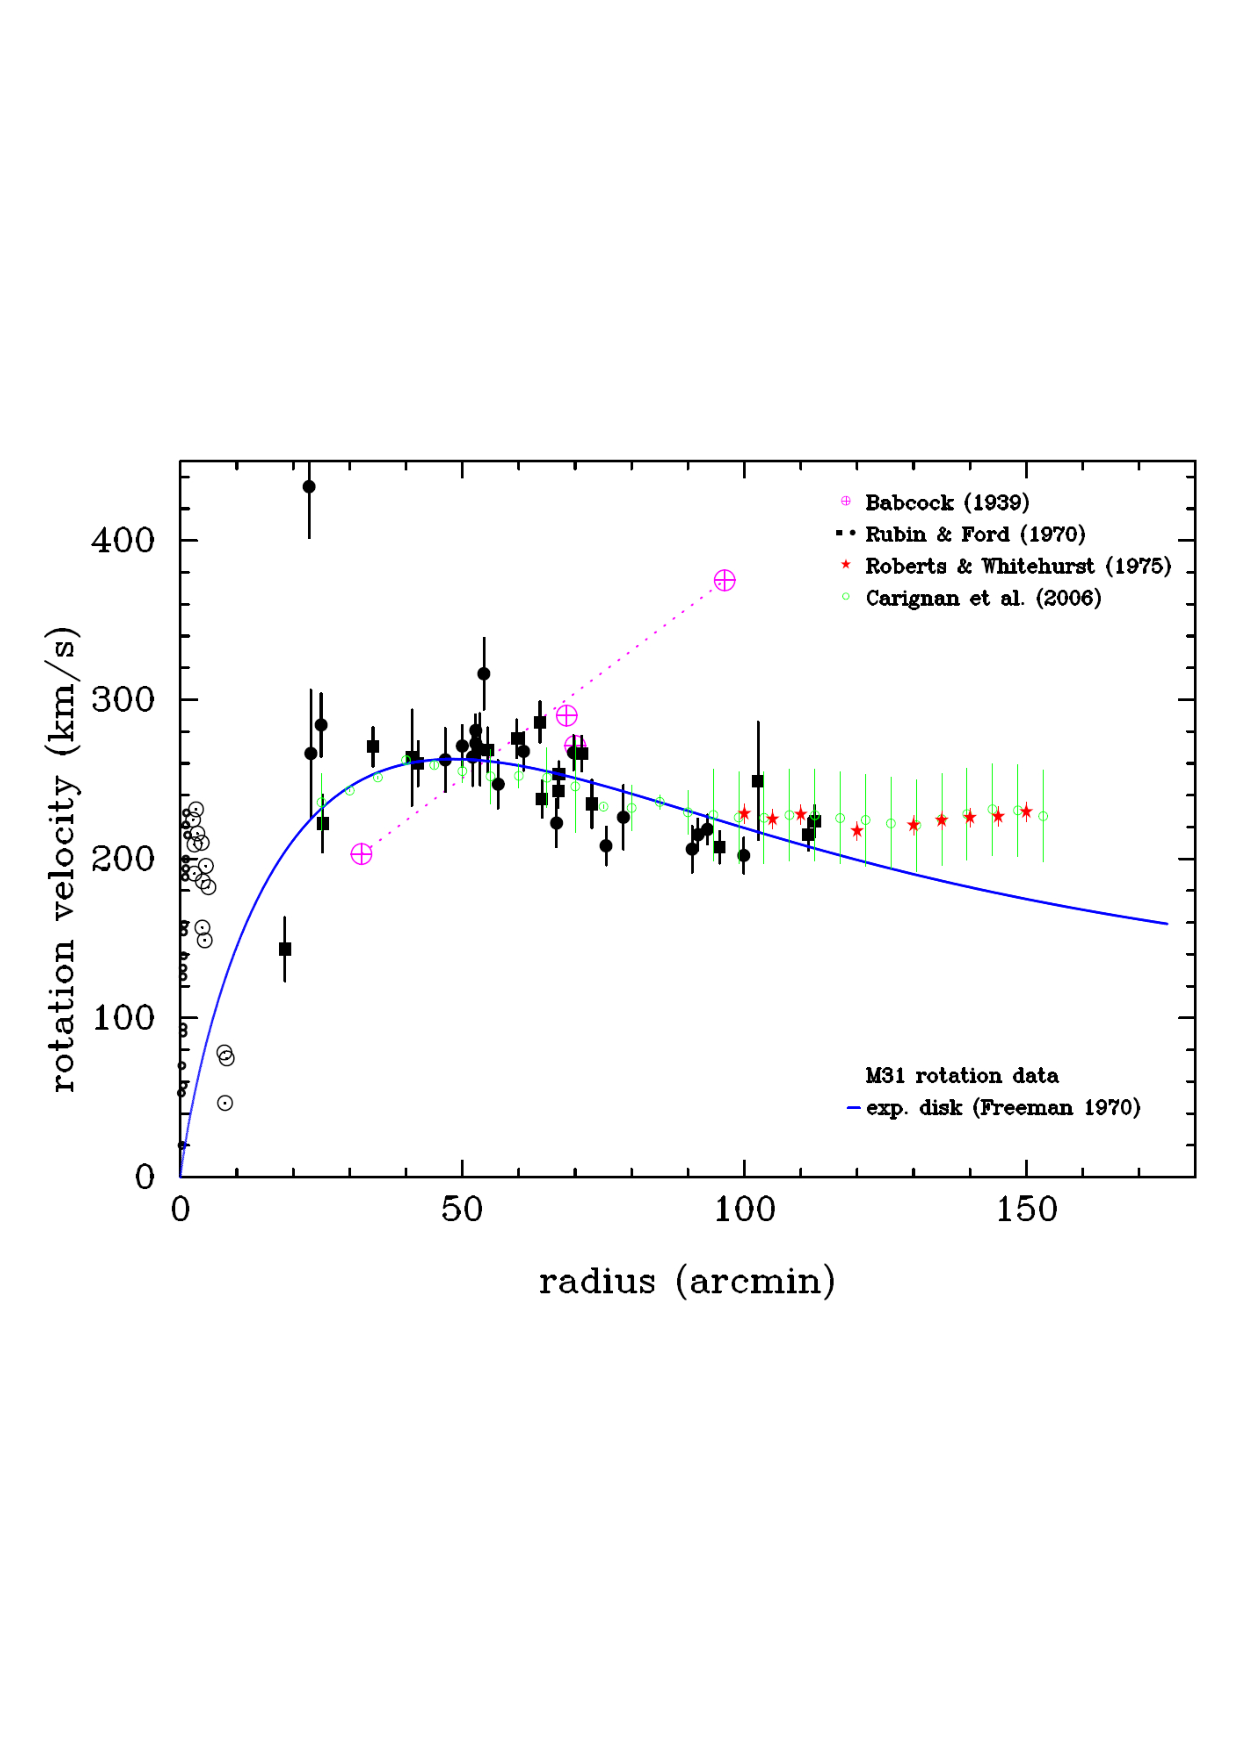
\includegraphics[width = 0.7\textwidth]{figures/DMOverview/m31-babcock-rf-rw.pdf}
	\caption[Galactic rotation curve data for M31.]{Rotation curve data for M31. The black points are from measurements (squares for the SW data, filled circles for the NE data, and open circles for the data in the inner parts – the presence of non-circular motions in the inner parts makes the modelling of those data uncertain). The red points are the 21-cm HI line data. The green points are 21-cm HI line data. The black solid line corresponds to the rotation curve of an exponential disc with a scale length according to the value given in Freeman, suitably scaled in velocity. 21-cm data demonstrates clearly the mass discrepancy in the outer parts. Figured reprinted from Ref.~\cite{HistoryofDM}.}
	\label{fig:DMOverview/NGC6503}
\end{figure}
\subsection{Gravitational lensing}\label{sec:DMOverview/GravLens}
The observed effect of gravitational lensing can be used to infer the total mass of an astronomical object by measuring the degree of deformation of light from background sources. An example of the effect gravitational lensing has on light from a distant galaxy is shown in the left panel of \autoref{fig:DMOverview/StrongGravLens}. Gravitational lensing was first described theoretically by Albert Einstein in 1936 \cite{GravLens}. The effect occurs when a massive object (lensing object) is situated in the line of sight between a distant source and an observer. Due to the gravitational field of the lensing object, light from the source deflects from its path, resulting in observable distortions such as magnification, image splitting, or the formation of arcs and rings.
When the lensing is strong enough to produce multiple images or highly distorted arcs, it is referred to as \textit{strong gravitational lensing}.
The degree of light deflection depends on the gravitational potential of the lensing object, which can be reconstructed by analysing the extent and geometry of the observed distortions \cite{Young2016}. 
The mass of the lensing object in the line of sight is compared with that of the observed baryonic matter (stars, dust, and gas), and the existence of dark matter is inferred to explain the discrepancy between the visible mass and lensing mass. 
Notable examples of clusters which exhibit such properties are the Coma Cluster \cite{Briel:1997hz}, Abell 370 \cite{Natarajan:2024iqm}, MACS J1206 \cite{GravLensPicture}, and the Bullet Cluster \cite{Clowe2006} shown in \autoref{fig:DMOverview/BulletCluster}.

\begin{figure}[h!]
	\centering
	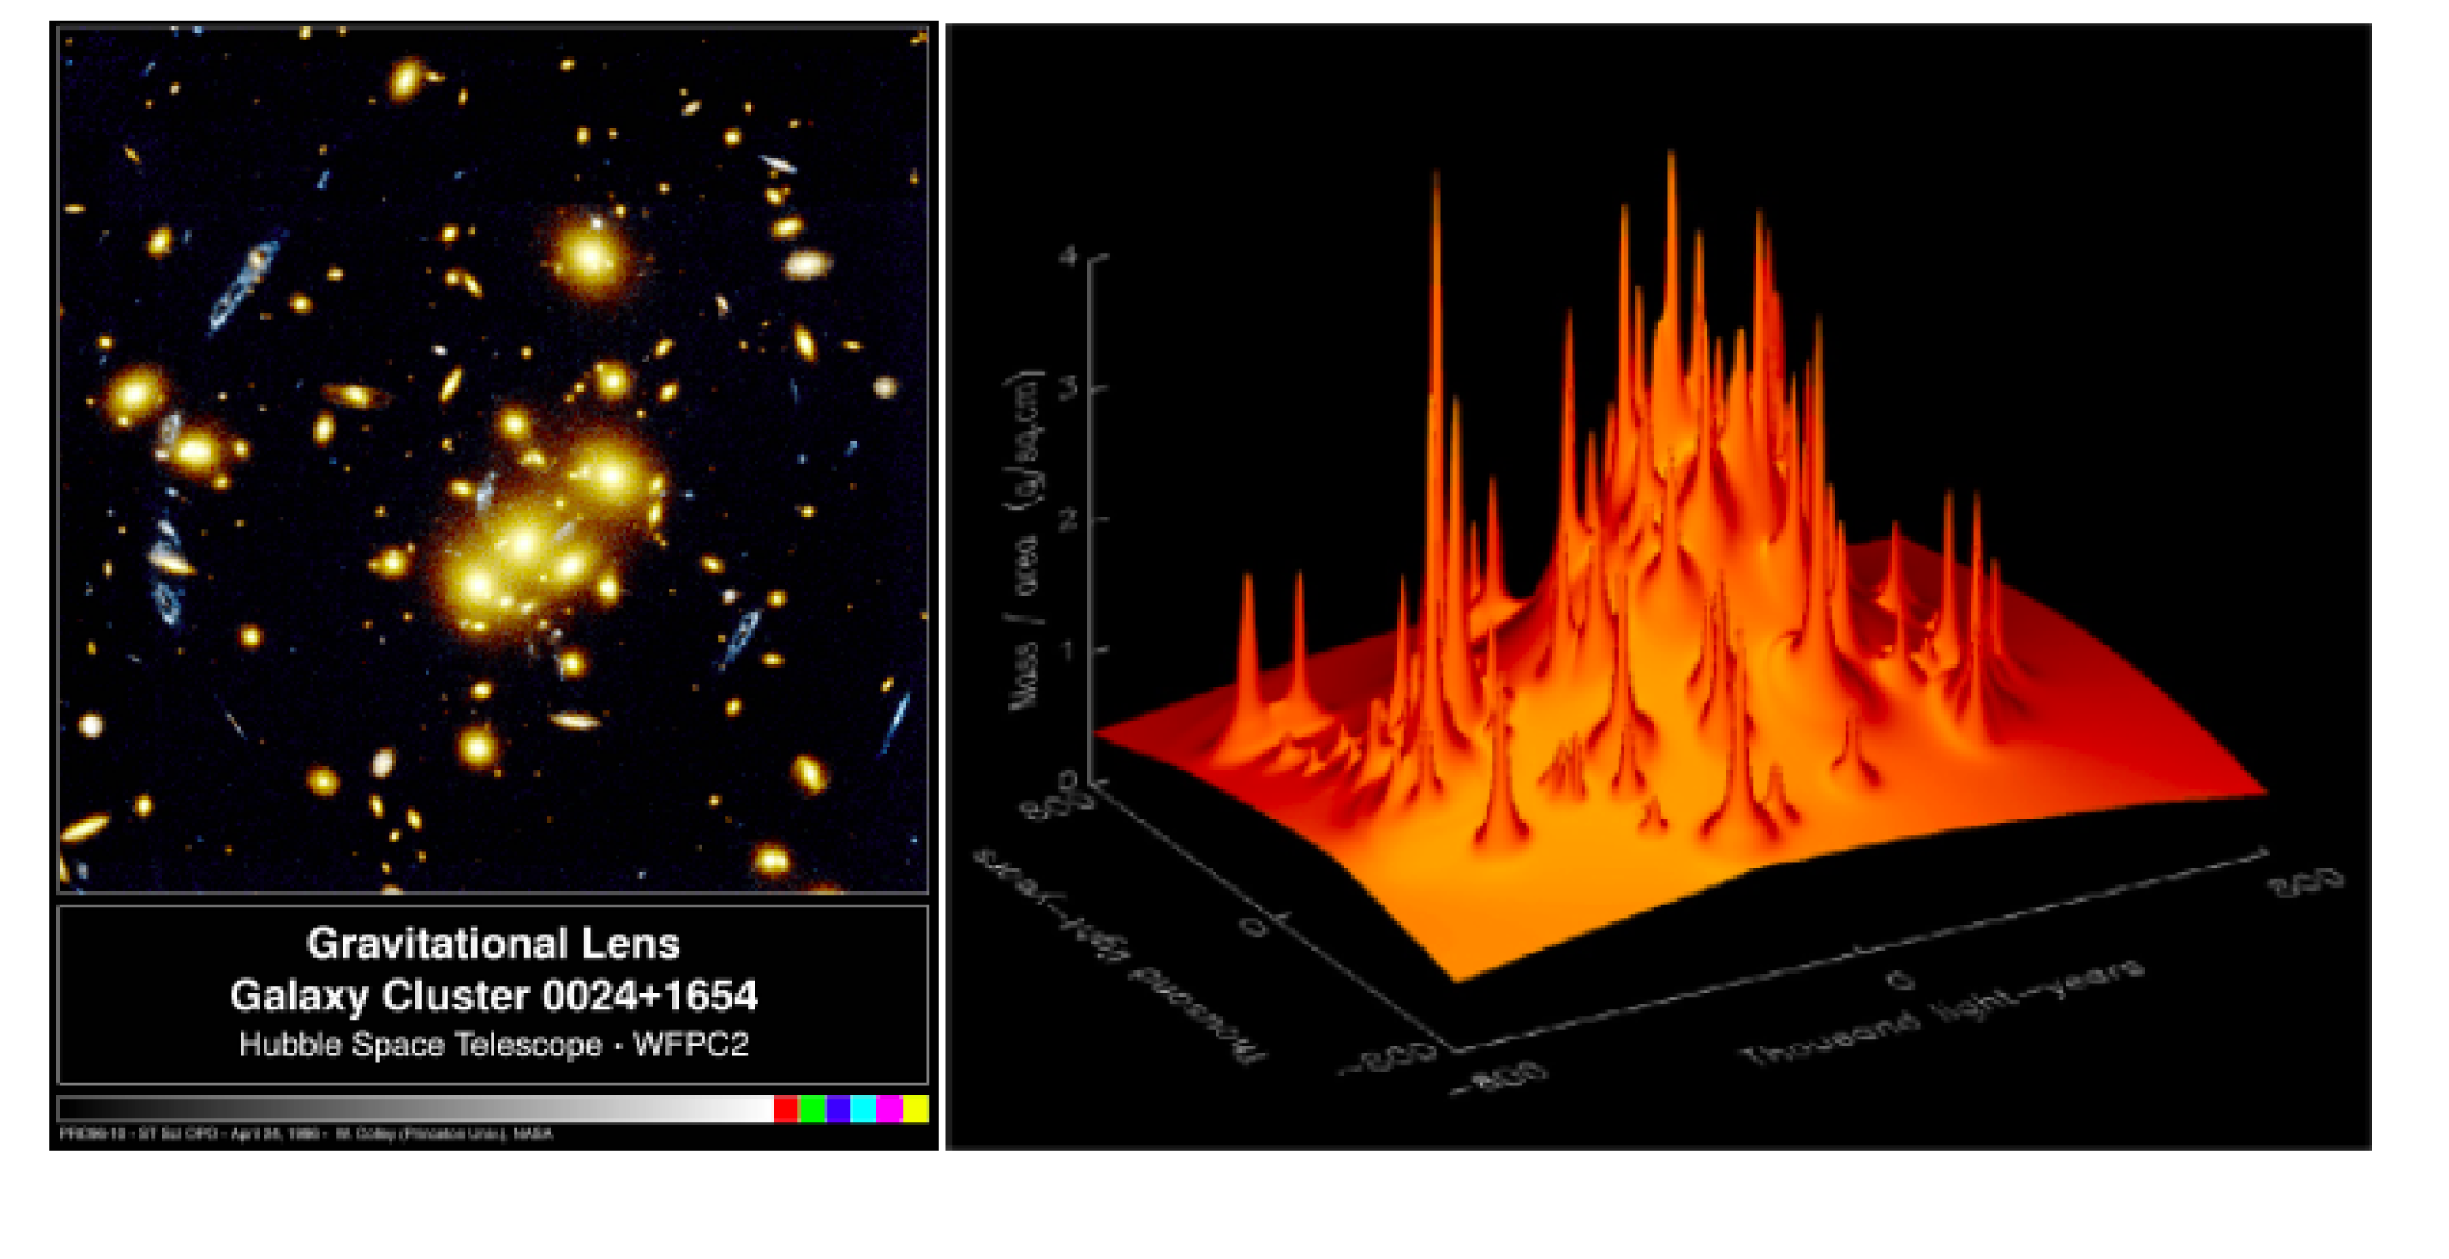
\includegraphics[width=0.9\textwidth]{figures/DMOverview/Strong_Grav_lens.png}
	\caption[Effects of gravitational lensing on multiple galaxies alongside the reconstruction of gravitational lensing effects.]{\textbf{Left:} An image from the Hubble Space Telescope where the foreground cluster of galaxies gravitationally lenses the blue background galaxy. \textbf{Right:} A reconstruction of gravitational lensing by a galaxy cluster. Baryonic matter within the cluster is represented by the sharp spikes, and the smooth background component corresponds to some non-visible mass. Figured reprinted from Ref.~\cite{Freese2009}.}
	\label{fig:DMOverview/StrongGravLens}
\end{figure}
\subsubsection{The Bullet Cluster}\label{sec:DMOverview/BulletCluster}
Observations of the Bullet Cluster (1E0657-558) made by the Hubble Space Telescope and the Chandra X-ray Observatory provide evidence for the existence of dark matter using gravitational lensing.
The Bullet Cluster consists of two galaxy clusters that have collided and are now moving apart. 
%A composite image of the cluster can be seen in \autoref{fig:DMOverview/BulletCluster}, where colour overlays represent the distribution of both luminous and total mass components. The blue regions in the image highlight the total mass distribution derived from gravitational lensing measurements, while the pink regions represent the hot, X-ray-emitting gas that contains the majority of the baryonic matter, such as gas and dust. 
Analysis of the X-ray data found that as the two clusters passed through one another, their gaseous components interacted strongly, colliding, slowing down, and heating up, producing intense X-ray emissions. This observation is shown in \autoref{fig:DMOverview/BCXrayData} where X-ray data has the lensing map overlaid.  Whereas measurements made using gravitational lensing indicated that the majority of the non-luminous portion of mass continued without disruption, the spacing between the mass peaks produced with the lensing analysis is shown using green contours in both images in \autoref{fig:DMOverview/BulletCluster}. The lensing mass peaks of the colliding clusters were compared with the X-ray peaks, and an offset was found \cite{Clowe_2004}. The offset found between the peaks is considered strong evidence for the presence of dark matter within the two colliding clusters. Clowe \textit{et al.}\cite{Clowe2006} applied Modified Theories of Newtonian Dynamics to the results to explain the Bullet Cluster formation, but were unable to fully explain the effect where the dark matter component in the regime was equal to the baryonic mass in the system. Therefore, the presence of dark matter in the cluster still holds true. The Bullet Cluster observations remain as the ``smoking gun'' in the pieces of evidence which support the existence of dark matter in the Universe.
\begin{figure}[h!]
     \centering
     \begin{subfigure}{0.49\textwidth}
         \centering
         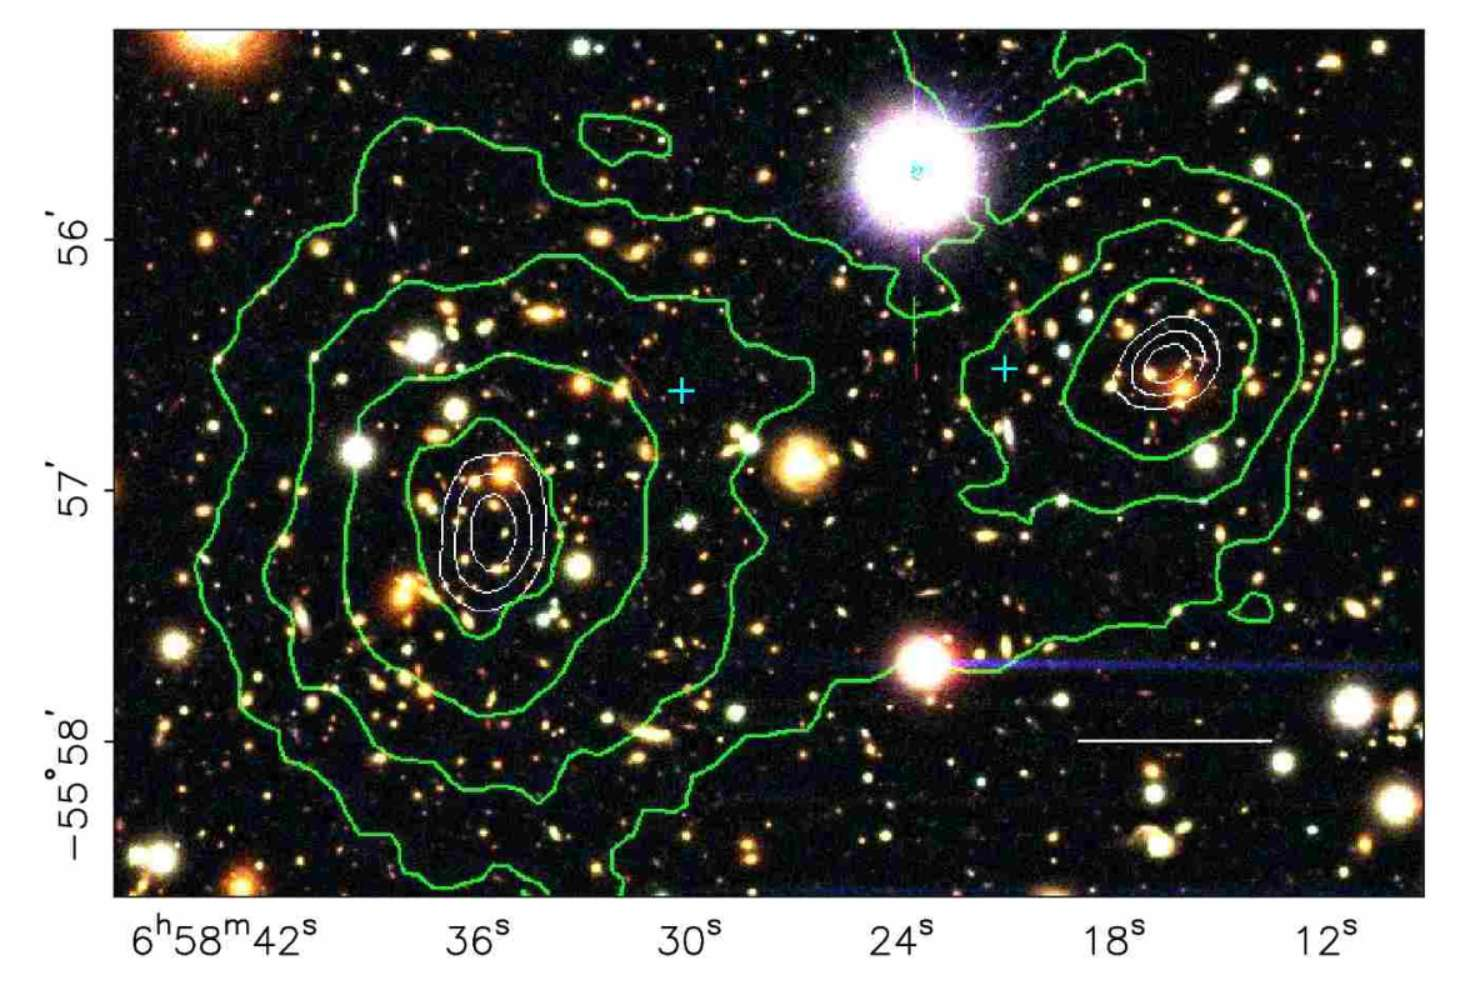
\includegraphics[width=\textwidth]{figures/DMOverview/f1a.new.jpeg2ps.png}
         \caption{}
         \label{fig:DMOverview/BCGravLensMap}
     \end{subfigure}
     \hfill
     \begin{subfigure}{0.49\textwidth}
         \centering
         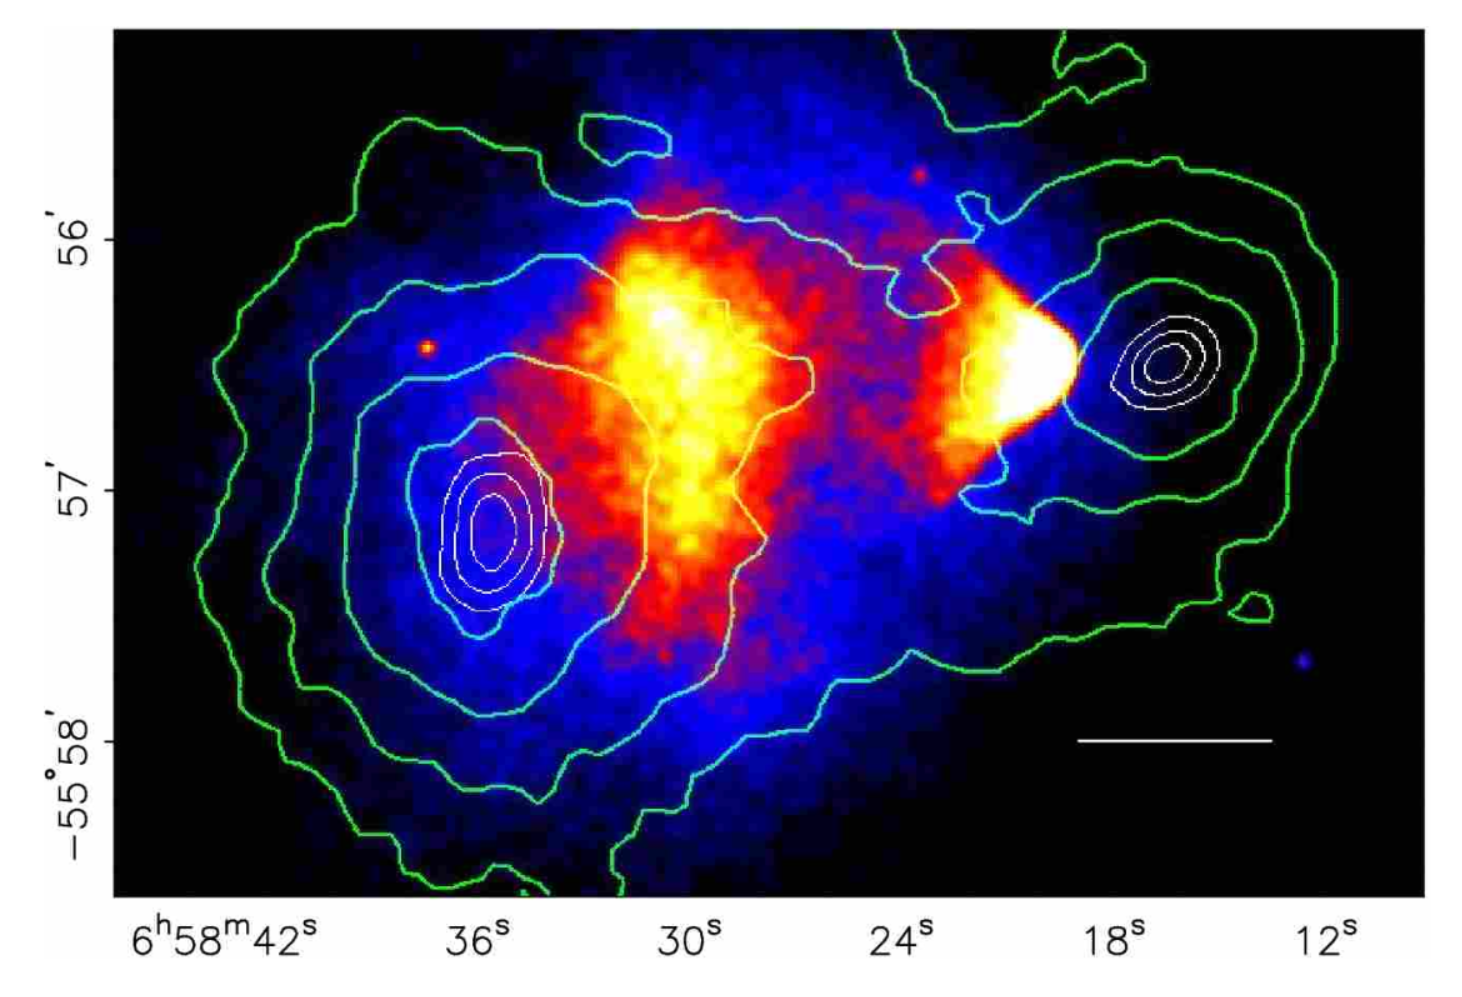
\includegraphics[width=\textwidth]{figures/DMOverview/f1b.new.jpeg2ps.png}
         \caption{}
         \label{fig:DMOverview/BCXrayData}
     \end{subfigure}
     \caption[The Bullet Cluster (1E0657-558) resulting from merger of two galaxy clusters.]{The Bullet Cluster (1E0657-558) resulting from merger of two galaxy clusters. \textbf{Left:}~A colour image from the Magellan images of the merging cluster, the white bar in the lower right of the image indicates 200~kpc at the distance of the cluster. \textbf{Right:}~An image from the Chandra X-ray Observatory. The green contours in both panels indicate the weak lensing reconstruction. Figures reprinted from Ref.~\cite{Clowe2006}.}
     \label{fig:DMOverview/BulletCluster}
\end{figure}

\subsection{The Cosmic Microwave Background}\label{sec:DMOverview/CMB}
The Cosmic Microwave Background (CMB) was first predicted by Ralph Alpher and Robert Herman in 1948 \cite{CMBprediction}, and subsequently discovered by Arno Penzias and Robert Woodrow Wilson in 1964 \cite{CMBDisco}. The CMB is relic radiation released after the Big Bang during the recombination epoch. The Universe was filled with an extremely dense, hot plasma of photons and charged particles. There was an initial rapid expansion of the Universe and then it continued to expand slowly over 380,000 years until the rate of expansion decreased as the temperature cooled, approaching the recombination epoch \cite{DMPrimer}. 

During this time, neutral particles were formed as free electrons bound to nuclei. The photons that were scattered from free electrons in the plasma state, which streamed freely through the Universe, were depleted due to this effect. The CMB is the result of the photons released during this \textit{last scattering} \cite{Cirelli:2024ssz}.

The CMB is not completely homogeneous and isotropic; however, it has a black body spectrum with a temperature of $(2.726\pm0.001)$~K \cite{Fixsen_2009}. Small fluctuations in the relic density after recombination are echoed in the relic temperature when gravity began to dominate matter. These variations are known as the CMB anisotropy. As a result, the CMB carries an imprint of the presence of dark matter, which is reflected in acoustic oscillations in the plasma where gravity provided the restoring force. The main observable is the CMB angular power spectrum shown in \autoref{fig:DMOverview/CMBPowerSpec}, which is obtained by performing a spherical harmonic Fourier transform of the CMB temperature shown in \autoref{fig:DMOverview/CMBImg}, and then computing the variance by averaging over the $2l+1$ orientations for each value of the angular momentum $l$ \cite{Cirelli:2024ssz}. The variations are compared to predictions of inflationary Big Bang cosmology, which yields information on the contents of the Universe. More precisely, the CMB peaks are due to acoustic oscillations of the baryon/photon fluid. The positions and amplitudes of the peaks represent the relative amount of dark matter with respect to normal matter, where only the latter undergoes acoustic oscillations. Global fits to the spectrum find that these oscillations and additional cosmological observations can be well produced by the Standard Model of cosmology, which includes dark matter ($\Lambda \text{CDM}$). The $x$-axis in \autoref{fig:DMOverview/CMBPowerSpec} is a rank of the multipole moments, which is inversely proportional to the angular coverage of the sky, where,
\begin{equation}
    l \approx\frac{180^{\circ}}{\theta_{\text{res}}(\text{degrees})},
\end{equation}
which is treated as a continuous variable \cite{Young2016}. The first peak at $l=200$ infers the total energy-matter density ratio to be $\Omega_{total}=1$. The size and location of the peak relate to the ``flat'' shape of the universe. The second peak, centred at $l\approx500$, informs how much baryonic matter is present in the universe. And the third peak at $l\approx700$ describes both the baryonic and dark matter components, where the difference between the second and third peak provides information on the density of dark matter in the early universe \cite{Young2016}.
\begin{figure}[!ht]
     \centering
     \begin{subfigure}{0.49\textwidth}
         \centering
         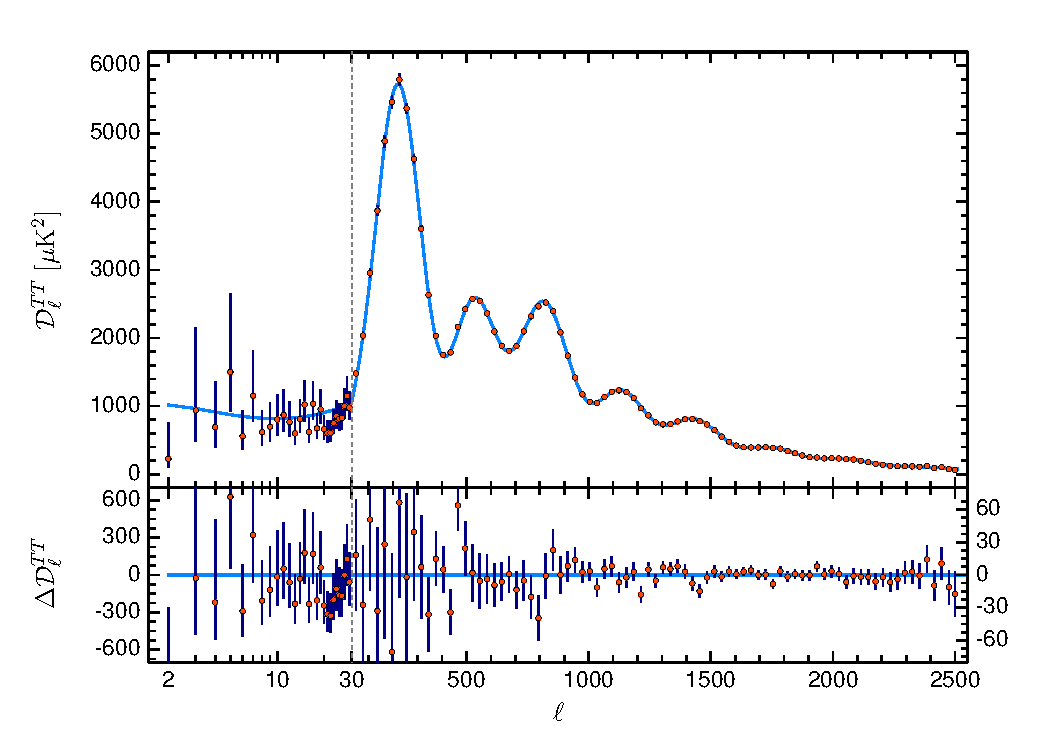
\includegraphics[width=\textwidth]{figures/DMOverview/coadded_TT.pdf}
         \caption{}
         \label{fig:DMOverview/CMBPowerSpec}
     \end{subfigure}
     \hfill
     \begin{subfigure}{0.49\textwidth}
         \centering
         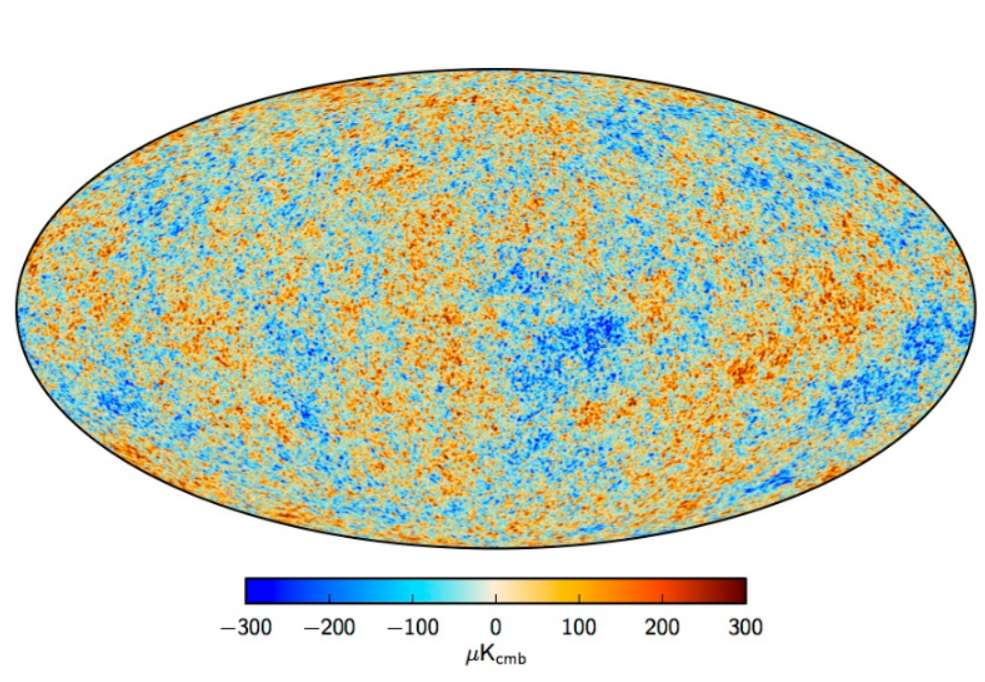
\includegraphics[width=\textwidth]{figures/DMOverview/CMBImg.png}
         \caption{}
         \label{fig:DMOverview/CMBImg}
     \end{subfigure}
     \caption[The power spectrum of the CMB acoustic peaks is extracted from the map of temperature anisotropies.]{The power spectrum of the CMB acoustic peaks (\textit{left}) is extracted from the map of temperature anisotropies (\textit{right}). The data points shown in blue are results from Planck 2018 \cite{Planck:2018vyg}. Figures reprinted from Ref.~\cite{Cirelli:2024ssz,Planck:2018vyg}.}
     \label{fig:DMOverview/CMB}
\end{figure}
\subsubsection{$\Lambda$CDM model}\label{sec:DMOverview/LambdaCDM}
The $\Lambda \text{CDM}$ model can be used to describe the measurements of the CMB well and requires the presence of dark matter in the Universe to support the result. The following six parameters are used in the model: the age of the universe; the density of atoms; the density of matter; the amplitude of the initial fluctuations; the scale dependence of this amplitude; and the epoch of first star formation \cite{LCDMparam}. This model incorporates high-sensitivity small angular resolution measurements in the infrared spectrum from the Planck space observatory \cite{2013Planck}, along with observations of early-universe fluctuations in the Cosmic Microwave Background (CMB) radiation obtained by the Planck \cite{WMAP}. The data from these sources is shown in \autoref{fig:DMOverview/CMBPowerSpec}, where the red line is the fitted $\Lambda \text{CDM}$ model. The most recent estimates from Planck 2018 \cite {Planck:2018vyg} allow a calculation of the mass-energy distribution in our Universe. The combined analysis results in a spatially-flat universe with a baryon density of $\Omega_{b}=0.049$, a dark matter density of $\Omega_{\text{DM}}=0.265$, and a dark energy density of $\Omega_{\Lambda}=0.686$.

\section{Alternatives to dark matter with the MOND}\label{sec:DMOverview/MOND}
One solution to explain the observations discussed in the preceding sections is to consider theories based on the Modification of Newtonian Dynamics (MOND). In 1982, Mordehai Milgrom considered the possibility that our understanding of the laws of gravitation on large scales where acceleration is extremely low was wrong and that there was no hidden mass in galaxies \cite{MOND}. A modification of Newtonian dynamics was proposed by Milgrom, where the force due to gravity would be scaled by a factor $a_0$ such that $F=\frac{ma^2}{a_0},$ where $a\ll a_0\sim 1.2\times10^{10}~\text{ms}^{-2}$ \cite{HistoryofDM}. Leading to the following formulation:
\begin{equation}
\begin{split}
    \frac{GMm}{r^2}&=\frac{mv^2}{a_0r^2}\\
    \Rightarrow v^2&=GMa_0
\end{split}
\end{equation}
This formulation states that a galaxy's orbital velocity would not be dependent on the distance from the galactic centre. The flatness seen in galactic rotation curves, shown in \autoref{fig:DMOverview/NGC6503}, could now be explained with the introduction of Milgrom's acceleration constant. However, this initial formulation had theoretical flaws in which momentum, angular momentum, and energy were not conserved. Additionally, MOND was not compliant with general relativity, so for MOND to be considered as an alternative to dark matter, both the classical and relativistic components needed to be addressed.
Through collaboration with Jacob Bekenstein, the pair attempted to resolve the issues of MOND \cite{Bekenstein1984}. In 2004, Bekenstein proposed a new theory, Tensor-Vector-Scalar
gravity (TeVeS), which would provide a solution to relativistic theories of MOND when applied to gravitational lensing \cite{TeVeS}. TeVeS was considered the leading theory to support MOND, but following the discovery of the Bullet Cluster by Clowe \textit{et al.}\cite{Clowe2006}. 
%The debate that MOND could be a viable solution to explain the observations shifted. 
An $8\sigma$ significance spatial offset of the centre of the total mass from the centre of the baryonic mass peaks could not be explained through modifications of the gravitational force law \cite{Clowe2006}. Many believe that the Bullet Cluster, taken together with other increasingly precise cosmological measurements, effectively brings the MOND hypothesis to an end \cite{HistoryofDM}. 

\section{Possible candidates for dark matter}\label{sec:DMOverview/Candidates4DM}
The evidence discussed so far in this chapter strongly indicates the existence of non-baryonic dark matter in our Universe. Based on early astrophysical observations, the new form of matter had to fulfil two criteria: it had to be non-luminous and have mass. But following further observations, physicists postulated that dark matter could arise from some form of undiscovered particle as opposed to some astrophysical material. The new particle should have the following properties:
\begin{itemize}
    \item Stable on timescales of $\mathcal{O}$(14 billion years), timescale of the Universe
    \item Non-baryonic
    \item Very weakly interacting via electromagnetic and strong forces
    \item Non-relativistic (cold) to allow clustering
    \item Very weak/no self interaction (except gravitational)
\end{itemize}
Considering these properties, many different theories have emerged that aim to describe a particle that is the dark matter, ranging in mass from $10^{-22}$~eV to many solar masses \cite{DMPrimer}. Some of these theories are shown in \autoref{fig:DMOverview/DMCandidates}. The following section will briefly review a small selection of these candidates.

\begin{figure}[h!]
    \centering
    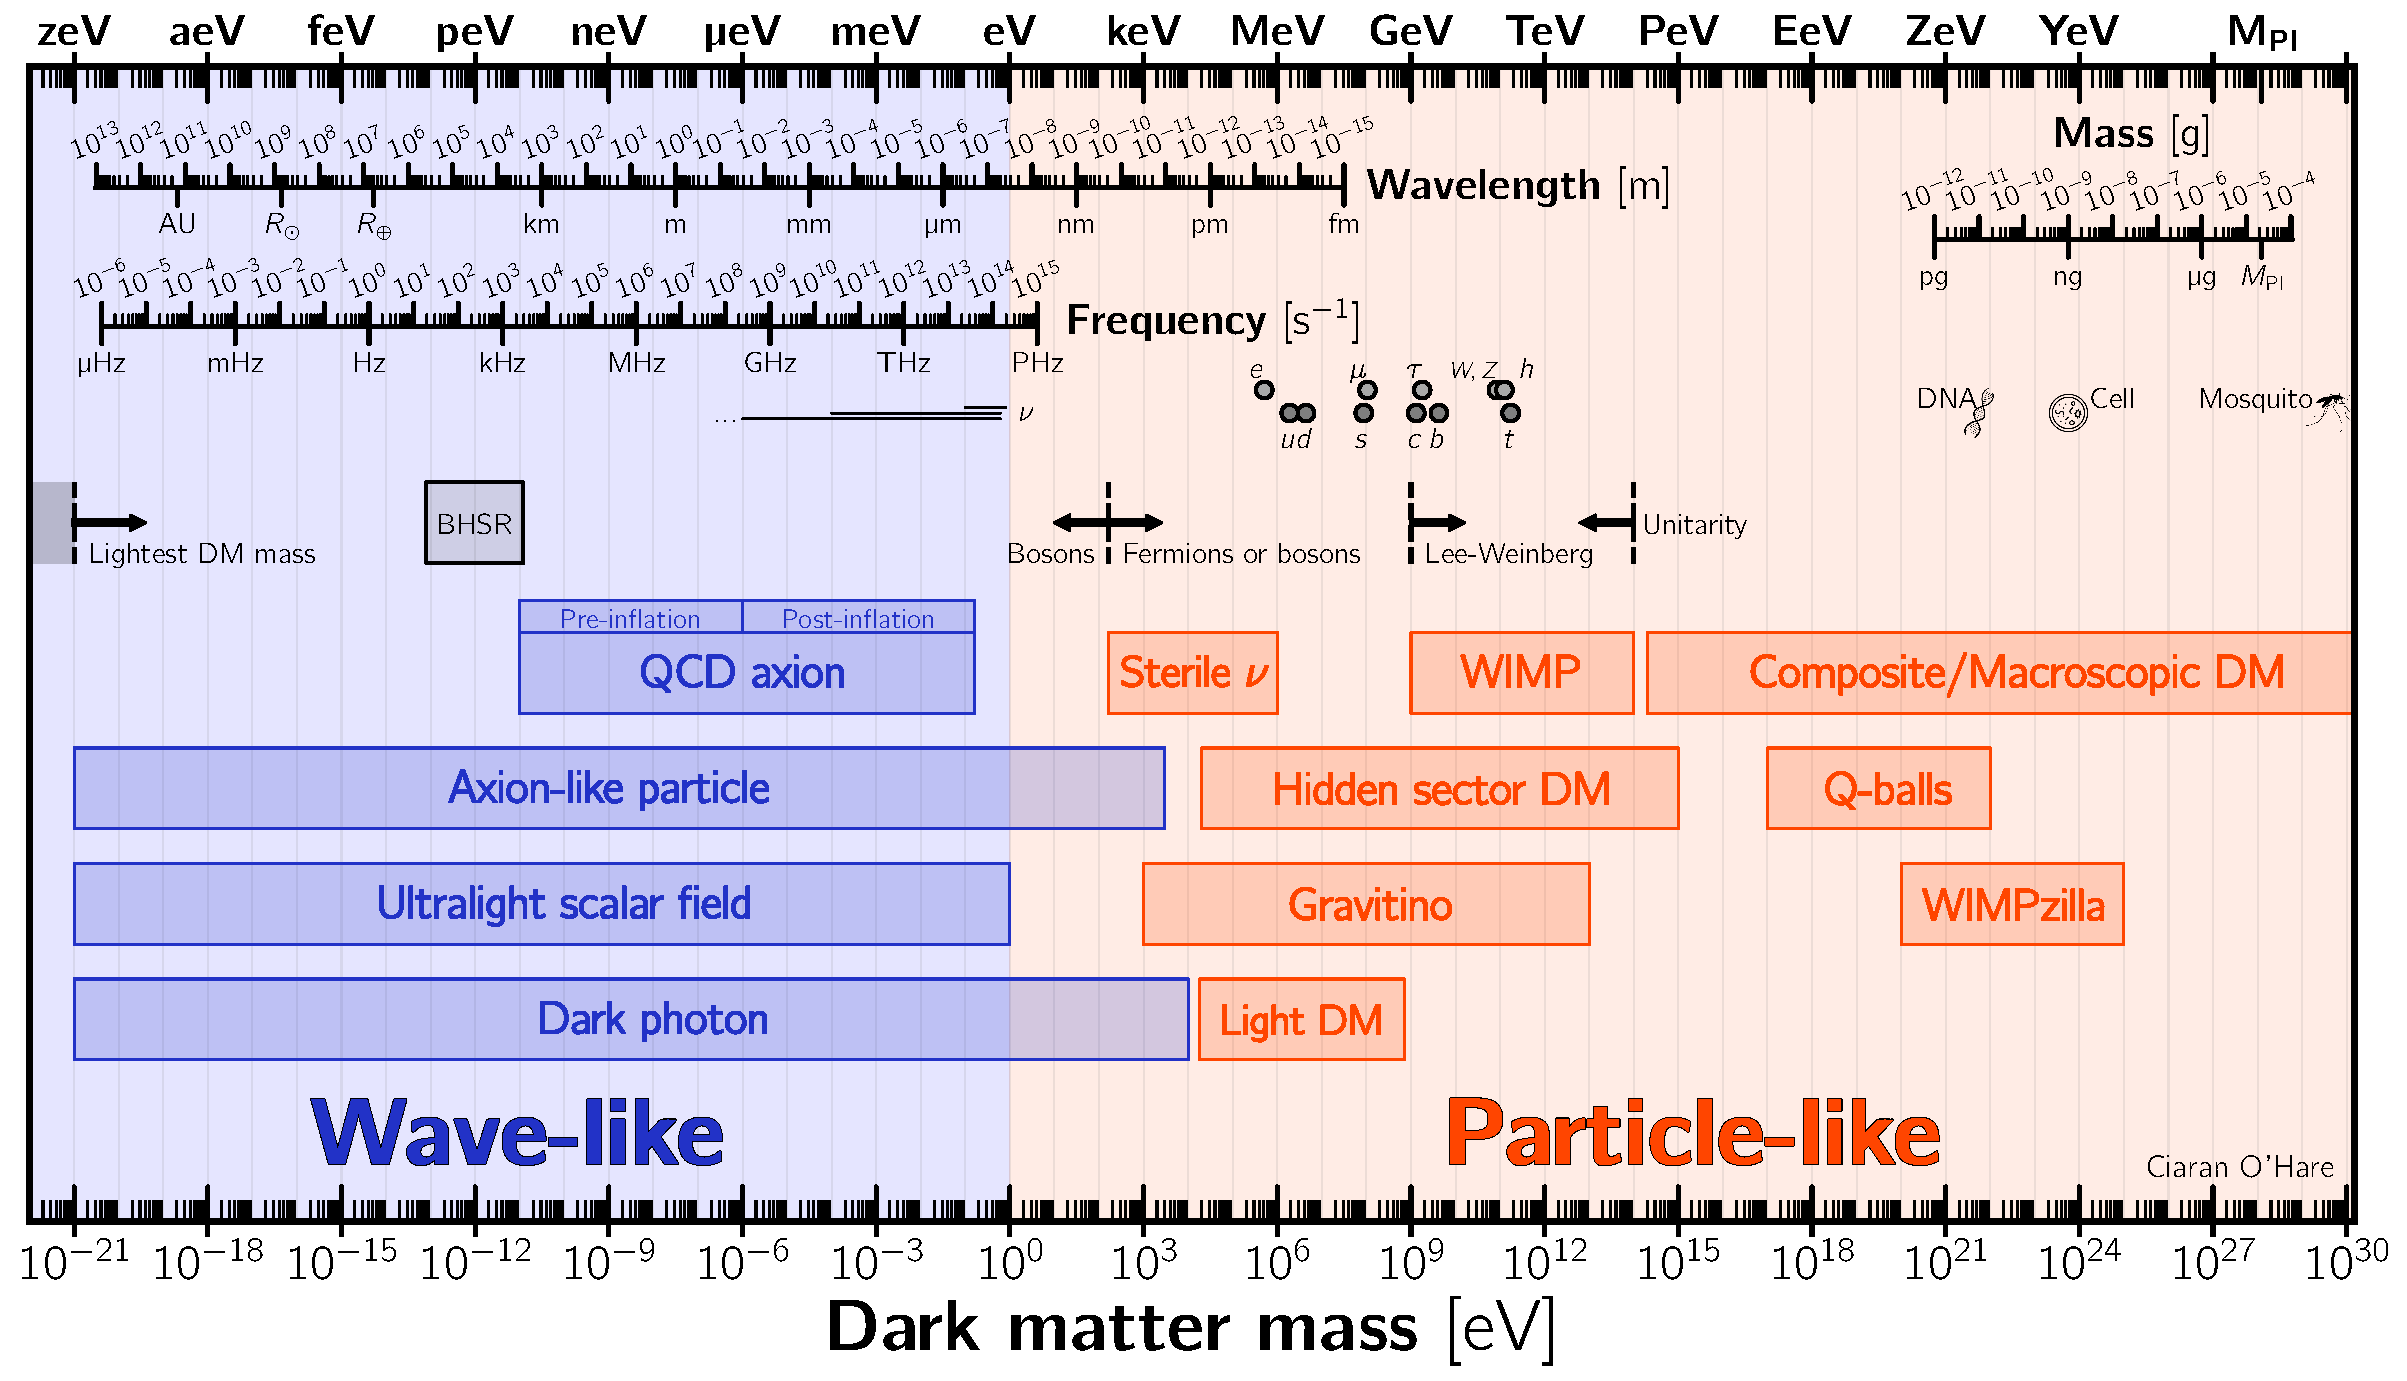
\includegraphics[width=\linewidth]{figures/DMOverview/Dark_matter_candidates.pdf}
    \caption[The current landscape of particle dark matter theories.]{The current landscape of particle dark matter theories. Most candidates can be categorized into two regimes ``particle-like'' or  ``wave-like'' which informs the particle mass and the subsequent ideal method of detection to search for these particles. Figure created by C. O'Hare and reprinted from Ref.~\cite{mwilliams:thesis}.}
    \label{fig:DMOverview/DMCandidates}
\end{figure}

\subsection{Neutrinos}\label{sec:DMOverview/Neutrinos}
One suitable candidate from the Standard Model to be considered as a dark matter candidate would be the neutrino. Being a stable, long-lived, and weakly interacting particle, the neutrino seems to fit the requirements outlined above. However, N-body simulations have shown that relativistic neutrinos found in the Standard Model do not allow the structure formation observed in the Universe \cite{White:1983fcs}. 
The hypothetical, sterile neutrino, proposed to explain the size of the neutrino mass, could provide a possible candidate for dark matter. When compared to the `hot' (relativistic) Standard Model neutrino, the sterile neutrino could either be a cold (always non-relativistic) or a warm (only relativistic in the early Universe) dark matter candidate, depending on its production mechanism. Thus far, experiments have produced results consistent with the Standard Model \cite{Boyarsky:2018tvu}, but research into this candidate is ongoing as the neutrino sector is probed further \cite{Krasnov:2019kdc}.


\subsection{Axions}\label{sec:DMOverview/Axions}
Axions are another form of particle that would be a candidate to solve the dark matter problem. The axion was first postulated to solve the ``strong CP (charge parity) problem'' in 1977 \cite{ConsvCP} due to the CP violation from the experimental bound on the neutrino dipole moment in quantum chromodynamics \cite{Hook:2018dlk}. Currently, constraints have been made on the possible axion dark matter mass to be between $10^{-6}$ and $10^{-2}$~eV \cite{Duffy:2009ig}. Experimental searches for the axion are ongoing through photon coupling. Notable examples of experiments are ADMX \cite{ADMX:2018gho} and CASPEr \cite{JacksonKimball:2017elr}. ADMX aims to detect the conversion of axions into microwaves, while CASPEr investigates axion-induced effects such as time variations in the nuclear dipole moment and nuclear spin precession.

\subsection{MACHOs}\label{sec:DMOverview/MACHOs}
A candidate at the other end of the mass scale could be Massive Astrophysical Compact Halo Objects (MACHOs), which emit little to no radiation. MACHOs could come in the form of neutron stars, black
holes, brown dwarfs, or unassociated planets, which could be used to explain the discrepancies observed in the cosmological observations discussed above. However, studies have shown that the majority of the dark matter density cannot entirely comprise of MACHOs \cite{Becker:2004ni,MicroLens}. Through a search for microlensing\footnote{Microlensing is a form of gravitational lensing which produces very small angular separations between the multiple images or changes in brightness, and the image they produce is too small to be resolved.} in the Large Magellanic Cloud (LMC), the MACHO Project found that MACHOs would constitute only $8\%$ of the dark matter halo in the LMC. This result ruled out a $100\%$ MACHO halo model \cite{MicroLens}.
The baryonic nature of the MACHOs additionally imposes constraints on their contribution to the total baryonic density observed through cosmological measurements and thus cannot be used to exclusively explain the mass-energy distributions in the Universe \cite{Planck2018}.

\subsection{WIMPs}\label{sec:DMOverview/WIMPs}
The Weakly Interacting Massive Particle (WIMP) is the final candidate to be discussed and is currently the most widely sought-after candidate for dark matter. The search for WIMPs is the primary science goal of the LUX-ZEPLIN experiment (see \autoref{chap:WS2024Result}). They are proposed as non-relativistic, heavy particles with interaction strengths on the scale of the weak force and are motivated by cosmological observations.

The relationship between the number density of dark matter and the WIMP self-annihilation cross-section is derived using conditions during the early Universe and assumes that there exist interactions between dark matter particles $\chi$ and Standard Model particles $p$, such that the process $\chi\chi\rightarrow pp$ occurs. Whilst the early Universe was in a hot, dense state, WIMPs were in thermal equilibrium with the cosmic plasma, given that the cross-section of this self-annihilation was sufficiently large. Big Bang Nucleosynthesis is used to predict the abundance of elements during this time, and it is natural to evaluate the evolving number density of dark matter using similar approaches \cite{Peebles:1991ch}. The evolution of the dark matter density in the expanding early universe can be described using a Boltzmann equation:
\begin{equation}\label{eqn:DMOverview/DMBoltz}
    \frac{dn_\chi}{dt}+3H(T)n_\chi=-\langle\sigma v\rangle\Bigl(n_\chi^2-n_{\chi_{eq.}}^2\Bigl),
\end{equation}
where $T$ is the temperature, $H$ is the Hubble rate, $\langle\sigma v\rangle$ is the thermally averaged dark matter pair annihilation cross-section, $n_\chi$ is the dark matter number density, $n_{\chi_{eq.}}$ is the equilibrium dark matter number density.

During the expansion of the Universe the temperature of the plasma cooled. Thermal equilibrium broke down at a critical temperature and density, this is when the dark matter yield is sufficiently different from its equilibrium yield. At this point, the dark matter number density is then constant with time and becomes a cold relic, i.e. ``dark matter freeze-out'' \cite{DMPrimer}. The result of \autoref{eqn:DMOverview/DMBoltz} shows that the dark matter density at which freeze-out occurs is inversely proportional to the dark matter annihilation cross-section. This result is shown in \autoref{fig:DMOverview/DMFreezeOut}. 
\begin{equation}
    \Omega_\chi h^2\approx\frac{3\times10^{-27}\text{cm}^3/\text{s}}{\langle\sigma v\rangle}
\end{equation}
Through the substitution of the relic abundance of dark matter observed, the expected cross-section is of order of a weak force interaction \cite{Arcadi:2017kky}. This mathematical coincidence is dubbed ``the WIMP miracle'' and has become a popular explanation for dark matter and it's existence in the Universe. Further discussion follows in \autoref{sec:DMOverview/DDFormalism} on the formalism required to detect WIMPs directly. %The LUX-ZEPLIN experiment's primary science goal is the direct detection of WIMPs.
\begin{figure}[h!]
    \centering
    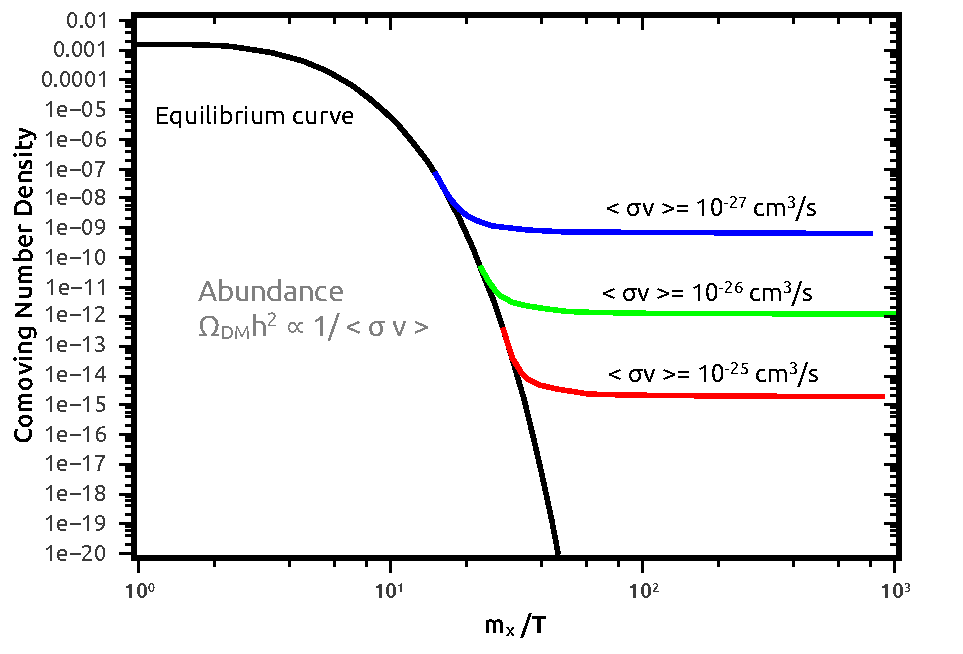
\includegraphics[width=0.7\linewidth]{figures/DMOverview/abundanceplot.pdf}
    \caption[The comoving number density as a function of the ratio $m_\chi/T$ with respect to the thermal freeze out.]{The comoving number density as a function of the ratio $m_\chi/T$ with respect to the thermal freeze out. The equilibrium curve corresponds to \autoref{eqn:DMOverview/DMBoltz}. It can be seen that the relic abundance is dependent on the dark matter self-annihilation cross-section. Figured reprinted from Ref.~\cite{Arcadi:2017kky}.}
    \label{fig:DMOverview/DMFreezeOut}
\end{figure}
\iffalse
The current dark matter density can be reproduced with the presence of WIMPs in the cosmological argument, this is known as the `WIMP miracle'\cite{DMPrimer}. 
During this time the annihilation rates of WIMPs producing Standard Model particles and the reverse process was in equilibrium. During the expansion of the Universe the temperature of the plasma cooled below that of the WIMP mass which led to the decoupling of WIMPs and baryonic matter \cite{DMProd}. During this time the production of WIMPs from Standard Model particles was suppressed, as such the WIMP density decreased exponentially with temperature. The dark matter relic density was reached when the annihilation rate of WIMPs became less that the Hubble expansion rate. Thus the cross-section required to detect a particle in the current density is of order of the weak interaction scale \cite{DMProd}. 
\fi

\begin{flushleft}
The candidates discussed in the sections above were not originally proposed to solve the dark matter problem, but were proposed to provide solutions to other models and theories in physics. The external motivation only strengthens the importance of the candidates.
\end{flushleft}

\newpage

\section{Searching for dark matter}\label{sec:DMOverview/DetectionOfDM}
The particle dark matter hypothesis can be tested via the following three mechanisms: production at particle accelerators; indirect detection by searching for signals from annihilation products; and direct detection via scattering on target nuclei. The possible dark matter, $\chi$, coupling to a Standard Model particle, P, is shown in \autoref{fig:DMOverview/detection_schem}. The following sections will review the different mechanisms as well as the current status of the searches so far. 
\begin{figure}[h!]
	\centering
	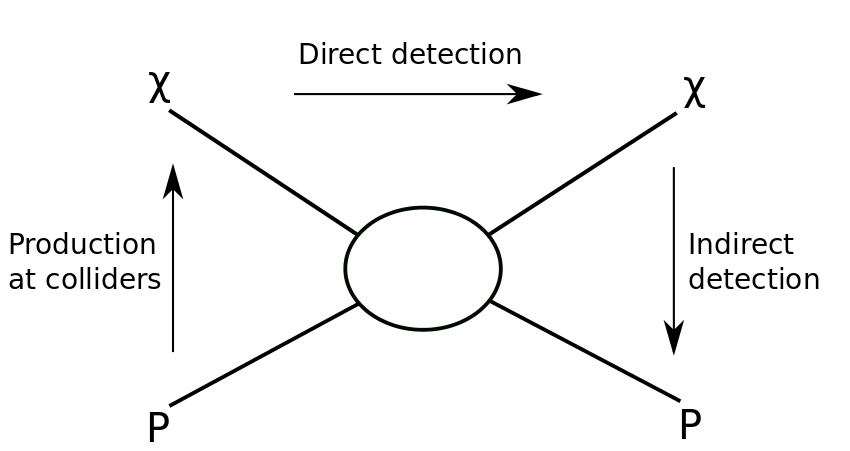
\includegraphics[width=0.7\linewidth]{figures/DMOverview/Detection_schematic.png}
	\caption[Schematic illustrating the possible dark matter detection methods.]{Schematic illustrating the three possible dark matter detection methods. Figured reprinted from Ref.~\cite{DirectDetection2015}.}
	\label{fig:DMOverview/detection_schem}
\end{figure}

\subsection{Dark matter production at particle colliders}\label{sec:DMOverview/DMProdColliders}
The production of dark matter, namely WIMPs, at particle colliders is a well-motivated approach as the electroweak scale is powerfully probed by colliders such as the Large Hadron Collider (LHC) at CERN \cite{Evans:2008zzb}. Since the start of the LHC in 2008, the ATLAS \cite{ATLAS:2008xda} and CMS \cite{CMS:2008xjf} experiments have searched for new particles in proton-proton collisions with a centre-of-mass-energy of 7~TeV to 13.6~TeV. Besides the discovery of the Higgs boson \cite{ATLAS:2012yve,CMS:2012qbp}, ATLAS and CMS experiments search for new particles by scanning the parameter space of different models of new physics, such as supersymmetry \cite{hteagle:thesis}.
Collider searches for dark matter can generally be divided into two categories: those that involve dark matter particles in the final state and those that do not. Both cases are dependent on the mass of the dark matter particle, $\chi$, and the mass of the mediator, which can be a known Standard Model (SM) particle (often but not exclusively the Higgs Boson) or an exotic mediator particle \cite{Penning:2017tmb}. 

If the dark matter particle mass is less than the mediator, then a WIMP pair is produced in the direction opposite to that of the visible particles. This results in a characteristic `mono-$X$' signature, where the `missing transverse energy', or more correctly `missing transverse momentum', ($E^{\text{miss}}_\text{T}$) and the visible particles $X$ are nearly back-to-back. The particle produced in this collision can be a multitude of particles such as $\gamma, q, g, W, Z, H$ and others. This mechanism is more commonly referred to as collider based dark matter production. An example event from a mono-$X$ search is shown in \autoref{fig:DMOverview/Mono-XEventViewer}.

\iffalse
\begin{figure}[h!]
    \centering
    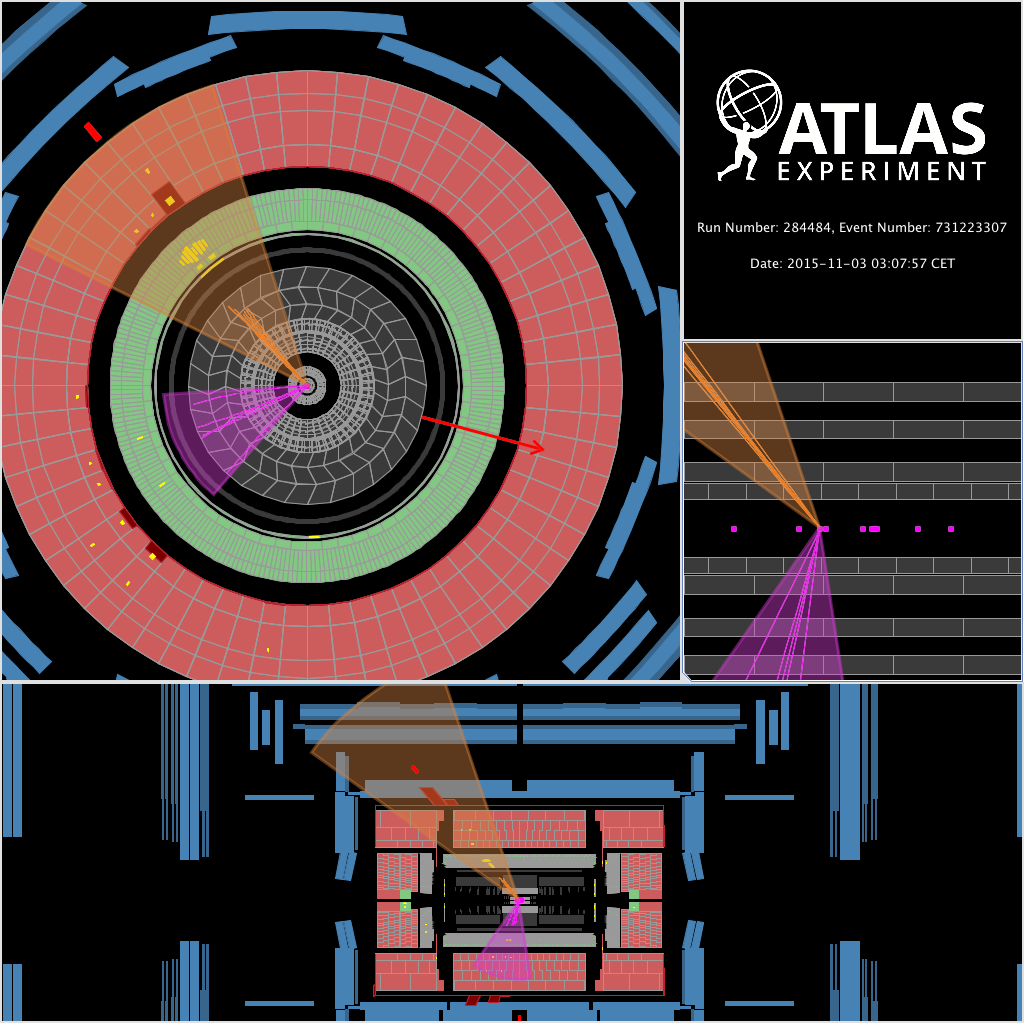
\includegraphics[width=0.6\linewidth]{figures/DMOverview/MonoXEventViewer.png}
    \caption[An event from a Mono-Higgs search from the ATLAS detector at the LHC.]{An event from a Mono-Higgs search from the ATLAS detector at the LHC. This event is characterized by $E^{\text{miss}}_\text{T}$~=~213~GeV (direction indicated with the red arrow) and two $b$-tagged small-R calorimeter jets that form a dijet system with $m_{jj}~=~120~\text{GeV}$ (shown in orange and magenta). Figure reprinted from Ref.~\cite{ATLAS:2016btj}.}
    \label{fig:DMOverview/Mono-XEventViewer}
\end{figure}
\fi

If the mediator is lighter than the dark matter, then the mediator becomes off-shell, then the processes proceeds via a virtual exchange and the process is suppressed. This is considered a search for a beyond the SM mediator \cite{hteagle:thesis}. If the hypothetical mediators couple to SM particles and the collider is powerful enough then the mediator could be produced in the annihilation of SM particles.  An example is the dijet analysis looking for a narrow peak in the invariant mass of the two jets, $m_{jj}$ \cite{Penning:2017tmb}.
So far results remain consistent with Standard Model expectations \cite{CMS:2017jdm,ATLAS:2016bek} and significant constraints on a number of dark matter models and masses have been made. A comparison between ATLAS limits with direct detection experiments is shown in \autoref{fig:DMOverview/ATLASDMSearch}.

\begin{figure}[!ht]
     \centering
     \begin{subfigure}{0.42\textwidth}
         \centering
         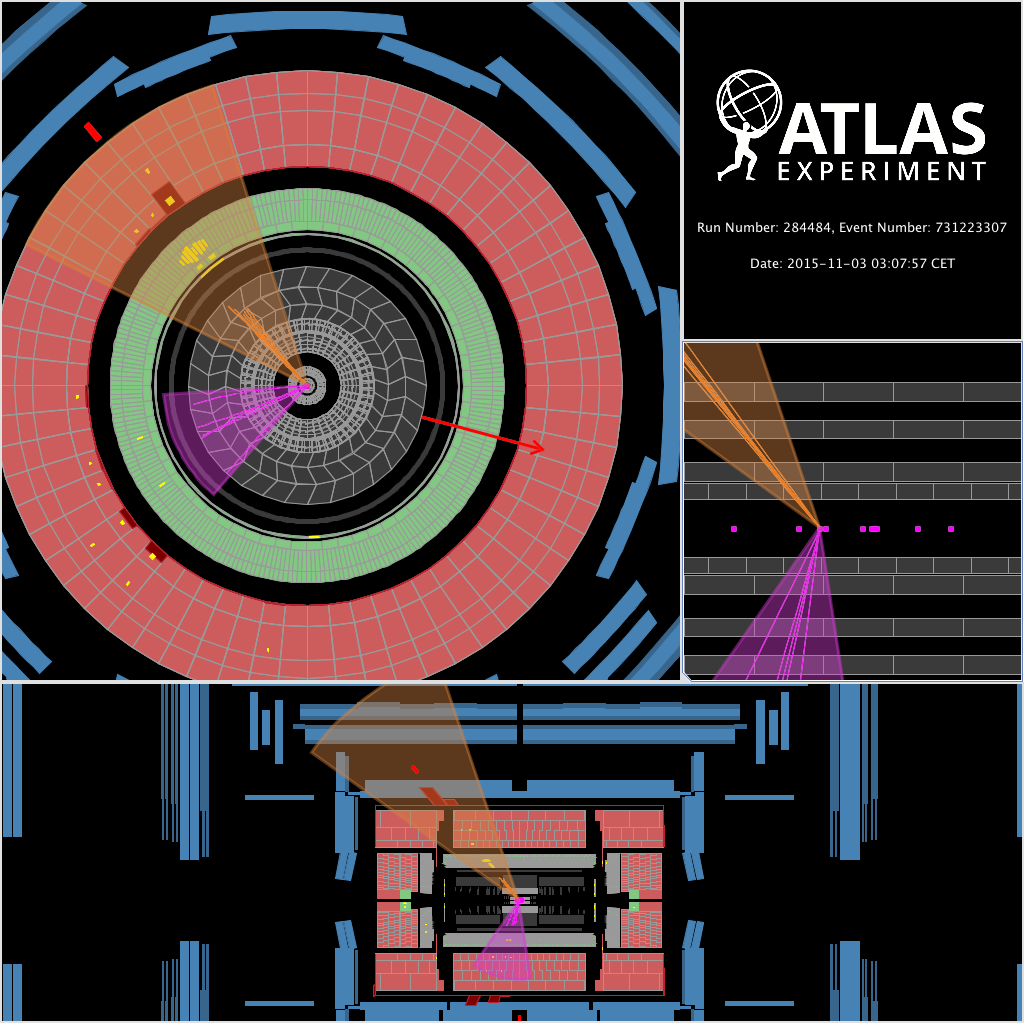
\includegraphics[width=\textwidth]{figures/DMOverview/MonoXEventViewer.png}
         \caption[An event from a Mono-Higgs search from the ATLAS detector at the LHC.]{}
         \label{fig:DMOverview/Mono-XEventViewer}
     \end{subfigure}
     \hfill
     \begin{subfigure}{0.56\textwidth}
         \centering
         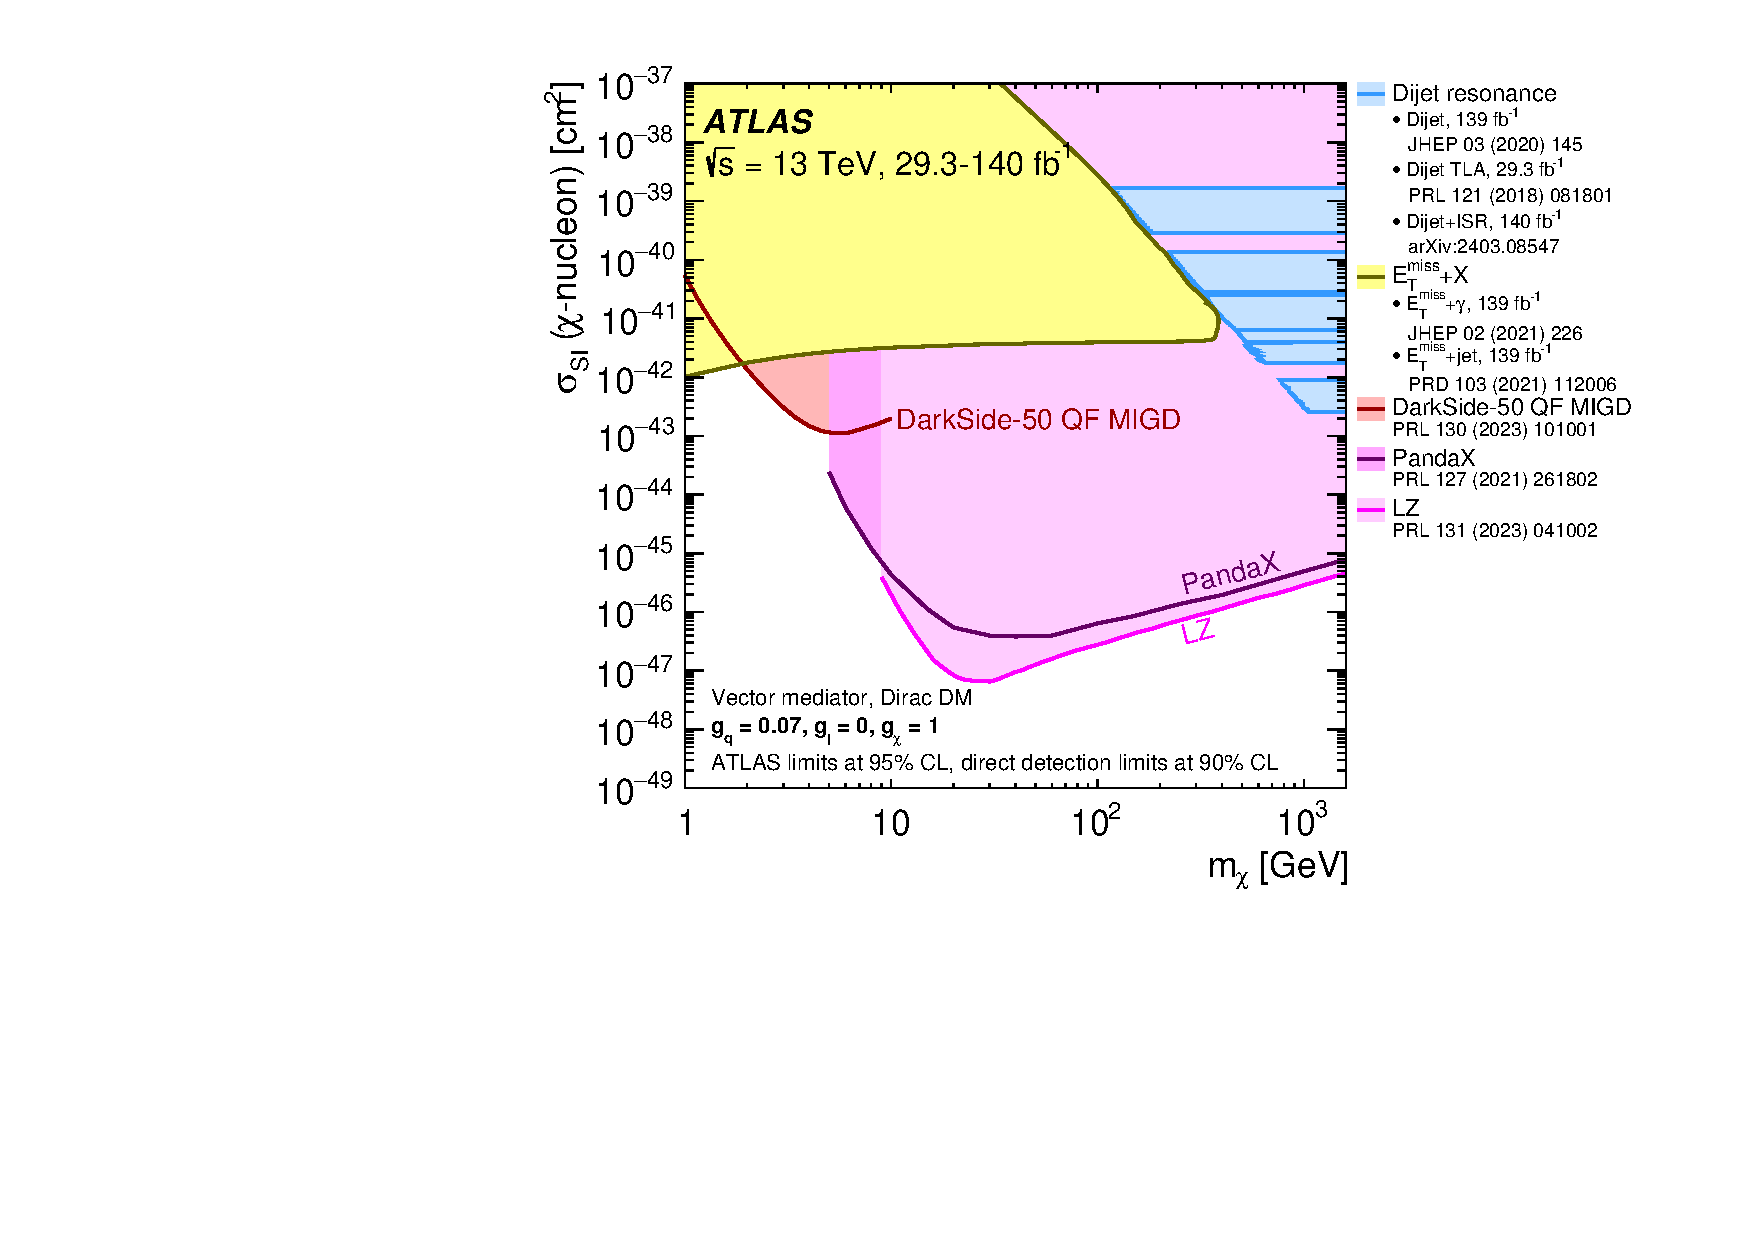
\includegraphics[width=\textwidth]{figures/DMOverview/ATLASDMSearch.pdf}
         \caption[Comparison between ATLAS limits with direct direction experiments in four scenarios]{}
         \label{fig:DMOverview/ATLASDMSearch}
     \end{subfigure}
     \caption[Dark matter searches at the LHC with the ATLAS detector.]{Dark matter searches at the LHC with the ATLAS detector. \textbf{Left:} An event from a Mono-Higgs search from the ATLAS detector at the LHC. This event is characterized by $E^{\text{miss}}_\text{T}$=213~GeV (direction indicated with the red arrow) and two $b$-tagged small-R calorimeter jets that form a dijet system with $m_{jj}~=~120~\text{GeV}$ (shown in orange and magenta). Figure reprinted from Ref.~\cite{ATLAS:2016btj}. \textbf{Right:} Comparison between ATLAS limits with direct direction experiments in four scenarios: V1 and V3 vector mediator couplings with spin-independent $\chi$-nucleon cross-sections, A2 axial-vector mediator coupling with spin-dependent $\chi$-proton cross-sections, and A4 axial-vector mediator coupling with spin-dependent $\chi$-neutron cross-sections \cite{ATLAS:2024kpy}. The conversion of the ATLAS results to the cross-section vs mass plane is detailed in Ref.~\cite{Boveia:2016mrp}. Figured reprinted from Ref.~\cite{ATLAS:2024kpy}.}
     \label{fig:DMOverview/ColliderTwoPanel}
\end{figure}

Dark matter searches at colliders are not restricted to the two mechanisms outlined above, some of which include long-lived particle searches \cite{Mitsou:2021tti}, new signatures and production modes \cite{Dienes:2021cxr,tcarter:thesis}, dark sectors searches \cite{Cohen:2017pzm,ajaspan:thesis}, novel instrumentation and different beams \cite{Feng:2017uoz,Batell:2014mga}. The collider will play a crucial role (if dark matter is kinematically accessible) when a discovery takes place first in either direct or indirect searches, as they will be well-suited to reproduce and measure dark matter under laboratory conditions.

\subsection{Indirect detection of dark matter}\label{sec:DMOverview/IndirectDM}
Based on evidence from observational cosmology, dark matter can gravitationally accumulate in halos around astronomical objects such as stars, galaxies, our Sun, and our galactic centre. These regions are potential sources of indirect dark matter signals. The increased dark matter density in these regions could produce a measurable particle flux of dark matter particles self-annihilating or decaying into Standard Model particles \cite{Strigari:2012acq}. The search for such signals is denoted as `indirect detection'. Examples of possible annihilation channels are:
\begin{equation}
    \chi\overline{\chi}\rightarrow\gamma\gamma,\gamma Z,\gamma H,q\overline{q},W^+W^-,ZZ,
\end{equation}
where some of the products decay further in $e^-e^+,\,p\overline{p},\,\gamma\text{-rays}$ and neutrinos \cite{DirectDetection2015}. For a given dark matter halo, the flux of the decay products arising from dark matter particle self-annihilations can be expressed as:
\begin{equation}\label{eqn:DMOverview/IndirectFlux}
    \frac{dN_i}{dAdtdE_i}=\frac{d\Phi_i}{dE_i}=\frac{1}{4\pi}\frac{\langle\sigma_Av\rangle}{2m^2_\chi}\frac{dN_i}{dE_i}\times\int_\Omega\int_{l.o.s}\rho^2_\chi(r)drd\Omega,
\end{equation}
where $i$ represents the particle type, $\Phi_i$ corresponds to the particle flux being measured, $\langle\sigma_Av\rangle$ is the thermally averaged product of the dark matter self-annihilation cross-section and the dark matter velocity, $dN_i/dE_i$ is the spectrum of species $i$ produced by the annihilations, $\rho_\chi$ is the dark matter density of the source, and $m_\chi$ is the dark matter mass \cite{PerezdelosHeros:2020qyt}. The integral is computed along the line of sight (\textit{l.o.s}) and is referred to as the $J$-factor and is source specific, requiring knowledge of the structure of the dark matter halo of the source being considered.

If signals from dark matter decay instead of annihilation are probed, then \autoref{eqn:DMOverview/IndirectFlux} must be modified slightly: $\rho_0^2$ reduces to $\rho_0$ as only one particle participates in a decay, whilst two are needed for annihilation. Likewise, the $m_\chi^2$ term in the denominator reduces to $m_\chi$ under the same reasoning; and what is probed is $1/\tau$ instead of $\langle\sigma_Av\rangle$, where $\tau$ is the candidate lifetime.
The flux of the products determined using \autoref{eqn:DMOverview/IndirectFlux} is translated into a limit on the velocity-averaged annihilation cross section $\langle\sigma_Av\rangle$ as a function of dark matter masses $m_\chi$. 

A consideration concerning the use of \autoref{eqn:DMOverview/IndirectFlux} must be made. The formalism only considers the spectrum from the source and does not consider the diffuse
cosmological contribution from all the sources along the line of sight. For searches within our galactic neighbourhood, this contribution can be neglected. However, it can be relevant for sources at extended distances or in analyses with poor angular resolution, and in such cases these effects need to be included \cite{PerezdelosHeros:2020qyt}. The effects are described further in Ref.~\cite{Beacom:2006tt,Ullio:2002pj}.

Many possible indirect detection mechanisms can be searched for, each with its own specific detection apparatus.
High-energy $\gamma$-rays are detected using atmospheric Cherenkov telescopes, which are pointed specifically in the direction of objects where large amounts of dark matter can be expected. The FERMI-LAT collaboration has reported an excess of $\gamma$-rays from the galactic centre of the Milky Way \cite{Fermi-LAT:2015sau}, however, it is unclear if the excess signal is from dark matter annihilations or point source backgrounds \cite{Boyarsky_2011}. However, FERMI-LAT data have been used to publish constraints on dark matter annihilation cross-section from a null result of a dwarf galaxy search \cite{Fermi-LAT:2015ycq}. Additional upper limits have been derived by a number of telescopes \cite{Aleksic:2013xea,HESS:2014zqa,VERITAS:2017tif}. 
Large neutrino detectors such as ANTARES \cite{ANTARES:2016xuh} and IceCube \cite{IceCube:2009iyf} can search for dark matter annihilation into neutrinos. Both experiments have placed constraints on the spin-dependent WIMP-proton cross-section. The mechanism considered is that WIMPs scatter off protons in the Sun, which results in a sufficient momentum reduction to be bound by the Sun's gravity. The WIMPs bound in this way would then result in the WIMP annihilation to neutrinos more frequently, in addition to other SM particles. The neutrinos produced via this mechanism are expected to have an order of magnitude higher energy than solar neutrinos \cite{Hooper:2025ohk,Super-Kamiokande:2020sgt}. The current status of indirect searches for dark matter with neutrinos from galaxies spans a large range of dark matter masses, as illustrated in \autoref{fig:DMOverview/DMAnnhillationCrossSection}.
\begin{figure}
    \centering
    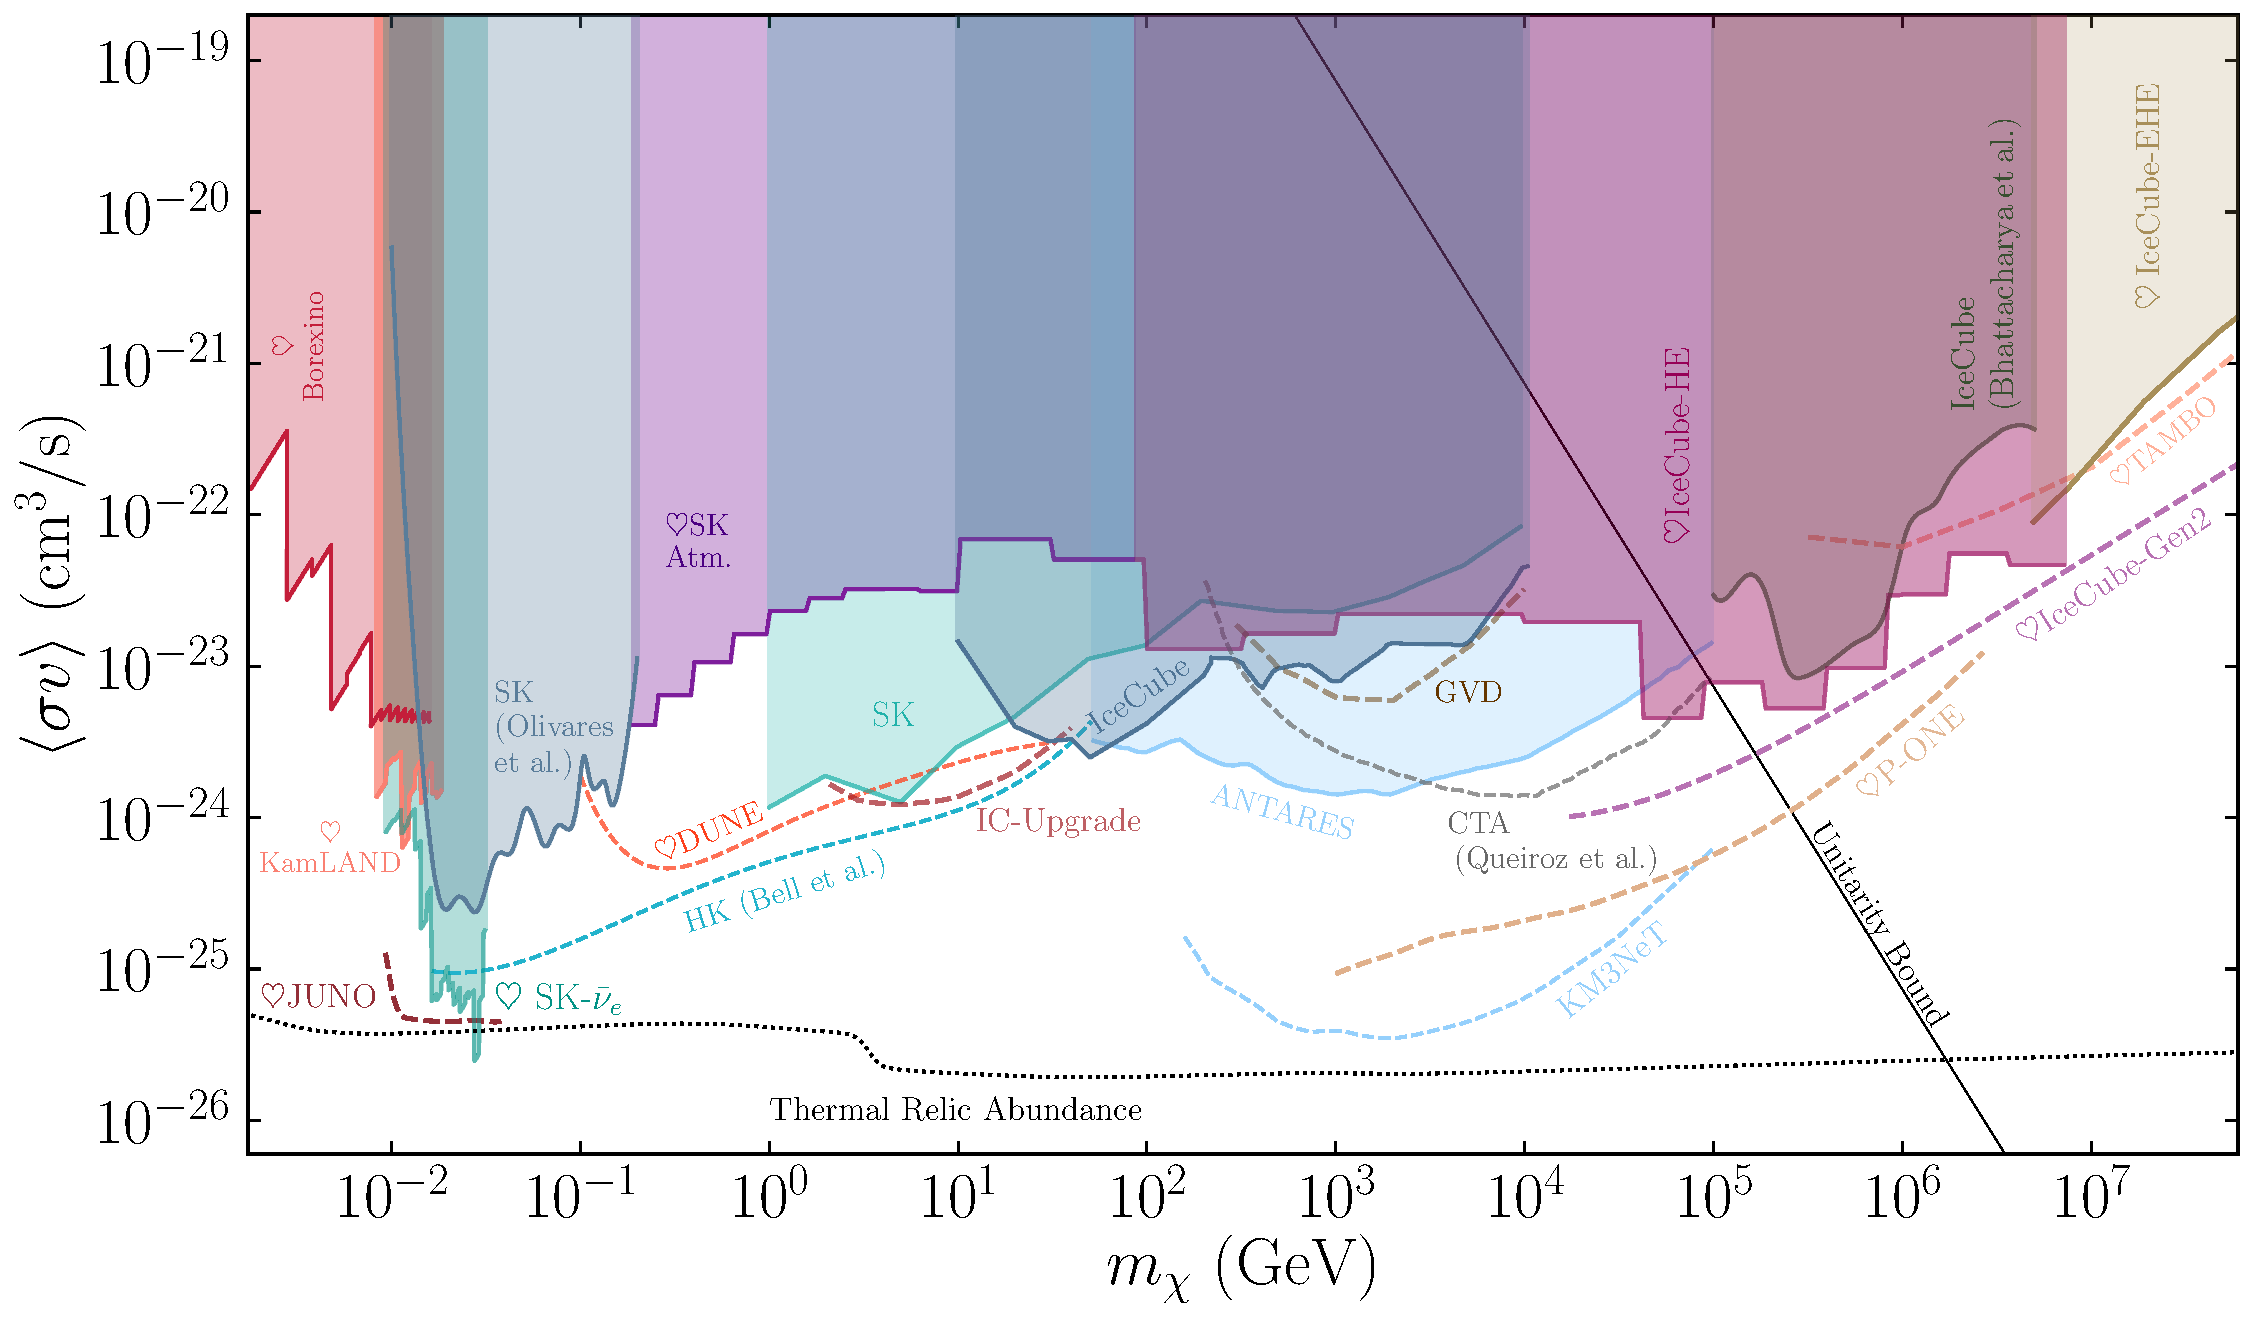
\includegraphics[width=\linewidth]{figures/DMOverview/MainPlot.pdf}
    \caption[Summary of results on the velocity weighted dark matter annihilation cross section from different indirect detection experiments.]{Summary of results on the velocity weighted dark matter annihilation cross section from different experiments. Limits are shown by solid lines, sensitivities for future facilities are shown by dashed lines, assuming five years of data taking. Analyses of public data performed by the authors of Ref.\cite{Arguelles:2019ouk} are additionally labelled with hearts. Reprinted from Ref.~\cite{Arguelles:2019ouk}.}
    \label{fig:DMOverview/DMAnnhillationCrossSection}
\end{figure}

\subsection{Direct detection of dark matter}\label{sec:DMOverview/DirectDetection}
The third mechanism to test the particle dark matter hypothesis is the direct detection of dark matter, where a dark matter particle scatters off a standard model particle, and the exchange of energy is measured in the laboratory. Direct detection experiments aim to observe nuclear or electronic recoils in target material resulting from such scatters.

\subsubsection{Direct detection formalism}\label{sec:DMOverview/DDFormalism}
A model to describe the rate $R$ of WIMP interactions in direct detection experiments can be determined by the movement of the Solar System through the Milky Way's dark matter halo. For ease of comparison between experiments, the local dark matter density $\rho_0$ is assumed to be between $0.2-0.4~\text{GeV cm}^{-3}$\cite{Green:2011bv}. As the Earth passes through the dark matter halo, WIMPs would elastically scatter off target nuclei with a cross-section dependent on velocity $\sigma_N\langle v\rangle$. The rate of interactions is proportional to the number of nuclei $N_T$ in the target, which leads to a rate of:
\begin{equation}
    R=n_\chi N_T\sigma_N\langle v\rangle=\frac{\rho_0M_T\sigma_N\langle v\rangle}{m_\chi m_A},
\end{equation}
where $n_\chi=\rho_0/m_\chi$ ($m_\chi$ is the mass of the WIMP) and $N_T=M_T/m_A$ ($M_T$ and $m_A$ are the total mass of the target and the atomic mass of the target, respectively). Direct detection experiments aim to measure the differential rate of dark matter interactions per unit recoil energy $E_\text{R}$ and target mass, expressed in terms of counts/kg/day/keV (a quantity referred to as a differential rate unit or \textit{dru})\cite{Cerdeno:2010jj}. 
For the WIMP case, a nuclear recoil would be observed with recoil energy $E_\text{NR}$. The differential event rate for a WIMP mass $m_\chi$ and a nucleus with mass $m_A$ is expressed as:
\begin{equation}
  \frac{dR}{dE_\text{NR}}=\frac{\rho_0}{m_\chi m_A}\int_{v_{min}}^{v_{esc.}}  v
  f(v) \frac{d\sigma_N}{dE_\text{NR}}(v,E_\text{NR})\, d v\,,
  \label{eqn:diff_rate}
\end{equation}
where $f(v)$ is the observed WIMP speed distribution in the laboratory frame, and $\frac{d\sigma_N}{dE_\text{NR}}(v,E_{NR})$ is the differential cross-section for the WIMP-nucleus elastic scattering per unit nuclear recoil energy for a given velocity $v$ \cite{jaalbers:thesis}.

The region of integration is defined between, the minimum WIMP velocity which can cause a nuclear recoil of energy $E_\text{NR}$: $v_{min}=\sqrt{(m_NE_\text{NR})/(2\mu_N^2)}$, where $\mu_N=m_\chi m_N/(m_\chi+m_N)$ is the WIMP-nucleus reduced mass; and the escape velocity of dark matter gravitationally bound in the Milky Way, $v_{esc.}\sim544~\text{km/s}$ \cite{OlcinaSamblas:thesis}. 

\iffalse
{\color{red}
The Standard WIMP Halo Model for local dark matter \cite{Evans:2018bqy} assumes a velocity distribution $f(\mathbf{v})$ of WIMP velocities $\mathbf{v}$ is a Maxwellian distribution limited by the same bounds defined for \autoref{eqn:diff_rate}:
\begin{equation}
    f(\mathbf{v})=\frac{1}{\sqrt{2\pi}\sigma}\text{exp}\biggl(-\frac{|\mathbf{v}|^2}{2\sigma^2}\biggl),
    \label{eqn:DMOverview/WIMPVelocitydist}
\end{equation}
where $\sigma=\sqrt{3/2v_c}$ relates the local circular speed and the speed dispersion. As the Earth moves with velocity $\mathbf{v_E}$ with respect to the galactic rest frame}
\fi

The WIMP-nucleus differential cross-section is defined as a combination of the spin-dependent (SD) and spin-independent (SI) contributions:
\begin{equation}
    \frac{d\sigma_N}{dE_\text{NR}}=\frac{m_N}{2\mu^2_Nv^2}\biggl(\sigma_\text{SD}F_\text{SD}^2(E_\text{NR})+\sigma_\text{SI}F_\text{SI}^2(E_\text{NR})\biggl),
\end{equation}
where the functions $F_\text{SD, SI}^2(E_\text{NR})$ are nuclear form factors and $\sigma_\text{SD, SI}$ are the spin-dependent and spin-independent cross-sections. The form factors account for the loss of coherence due to greater momentum transfer, $q=\sqrt{2m_NE_\text{NR}}$, leading to a suppression in event rate for heavy WIMPs \cite{Cerdeno:2010jj}. The SI form factor is often expressed in the form of the Helm form factor \cite{edfraser:thesis}:
\begin{equation}
    F_\text{SI}^2(q)=\biggl(\frac{3j_i(qR_1)}{qR_1}\biggl)^2\text{exp}(-q^2s^2),
\end{equation}
where the nucleus is represented as a solid sphere of radius $R_1$ surrounded by a skin of thickness $s$ and $j_i$ is the first spherical Bessel function. The form factor is target dependent and this effect is shown in \autoref{fig:DMOverview/SIFF} for the spin-independent case.
The WIMP-nucleon cross-sections, e.g. $\sigma_\text{SI}$ (see \autoref{eqn:DMOverview/WIMP-nucleon_cross-sectionSI}), enable comparison between experiments with different target materials and are calculated by analysing the scalar spin-independent (SI) and vector spin-dependent (SD) couplings of WIMP candidates to quarks, which are prompted to WIMP-nucleon cross-sections using hadronic matrix elements \cite{edfraser:thesis}.
\begin{equation}\label{eqn:DMOverview/WIMP-nucleon_cross-sectionSI}
    \sigma_\text{SI}=\biggl(\frac{\mu_N}{\mu_n}\biggl)^2A^2\sigma^\text{SI}_n
\end{equation}
Here $A$ is the atomic number of the target and $\mu_n$ is the reduced WIMP-nucleon mass. Therefore, the spin-independent WIMP-nucleon cross-sections are enhanced by heavier nuclei; this effect is shown in \autoref{fig:DMOverview/SINuclearRecoilRate}. The spin-dependent is more complex and is not shown; however, it is not dependent on $A^2$, and is dependent on the total nuclear spin, $J$ \cite{OlcinaSamblas:thesis}.

\begin{figure}[!h]
     \centering
     \begin{subfigure}{0.49\textwidth}
         \centering
         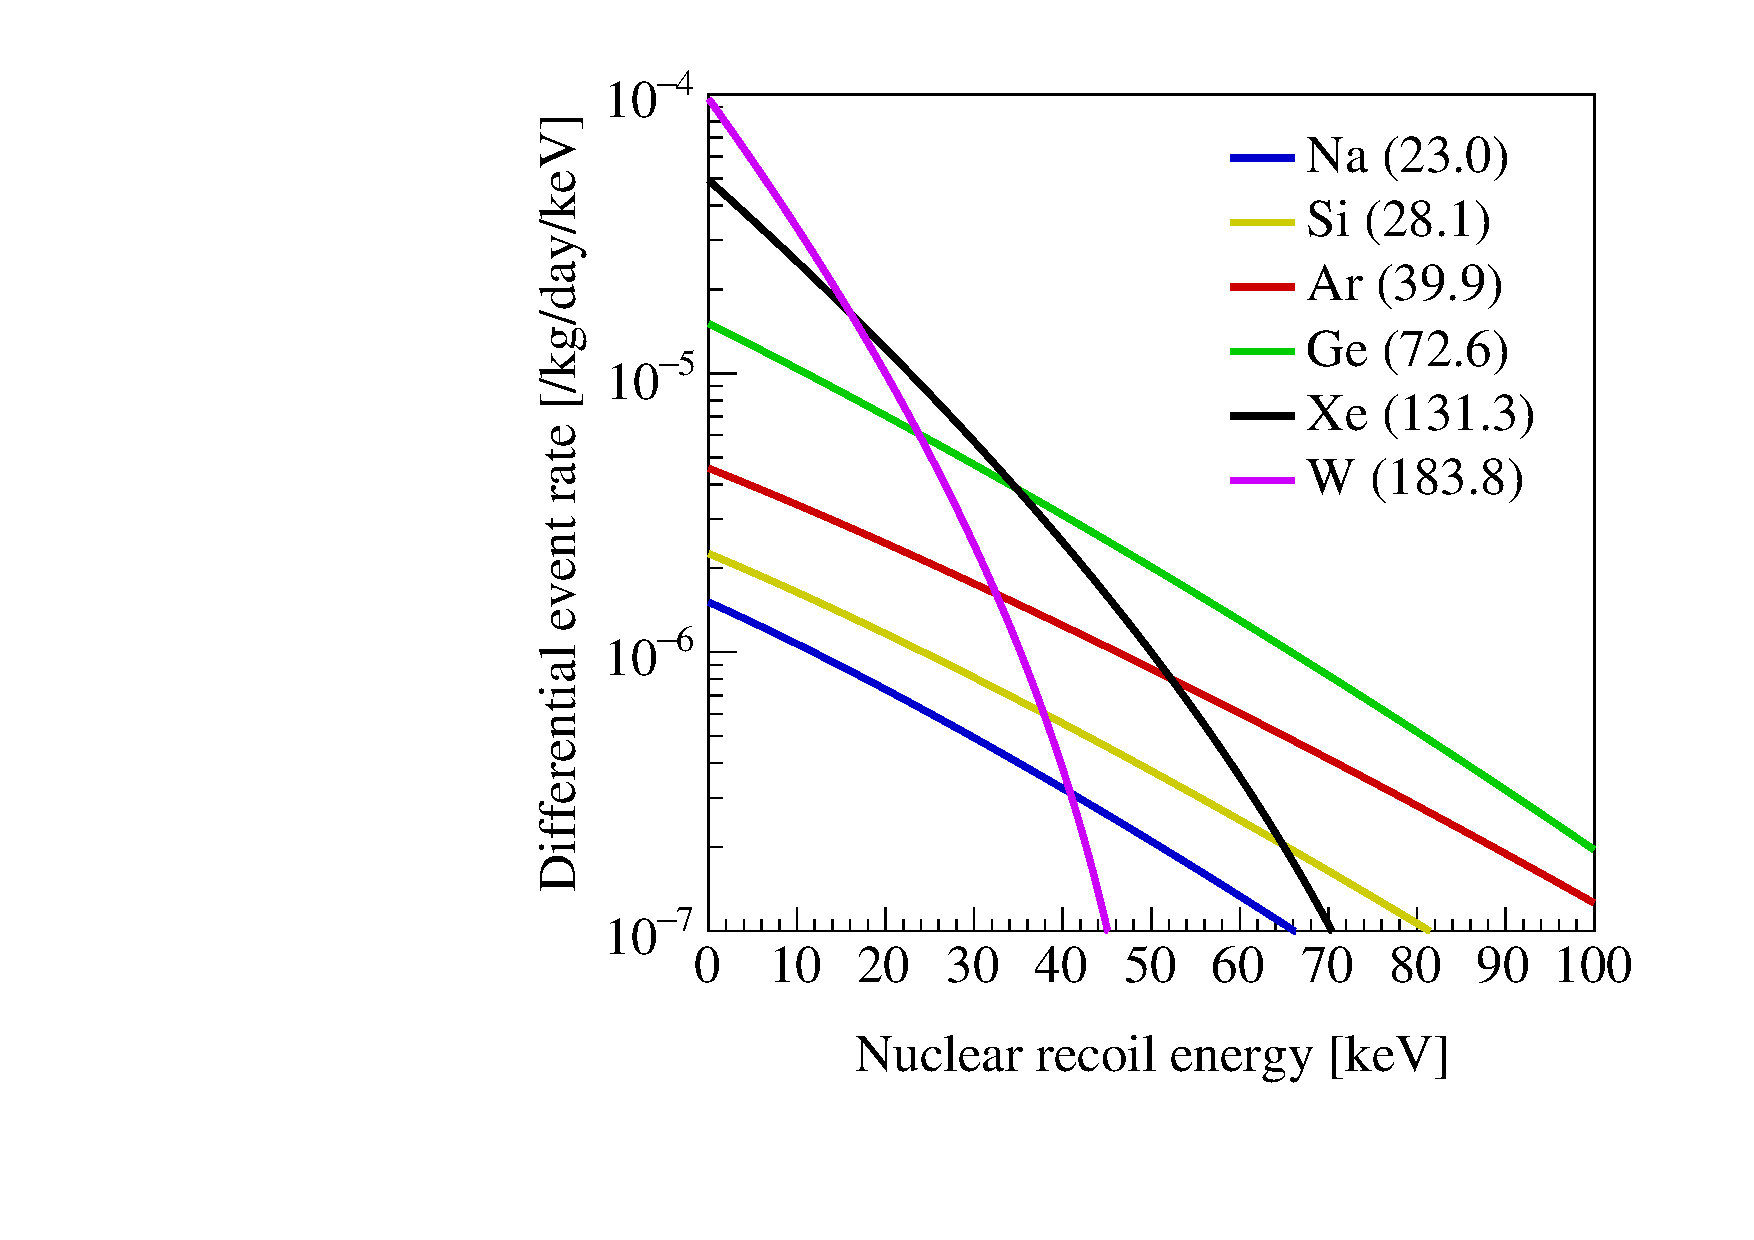
\includegraphics[width=\textwidth]{figures/DMOverview/wimp_event_rate_si_m100.pdf}
         \caption{}
         \label{fig:DMOverview/SINuclearRecoilRate}
     \end{subfigure}
     \hfill
     \begin{subfigure}{0.49\textwidth}
         \centering
         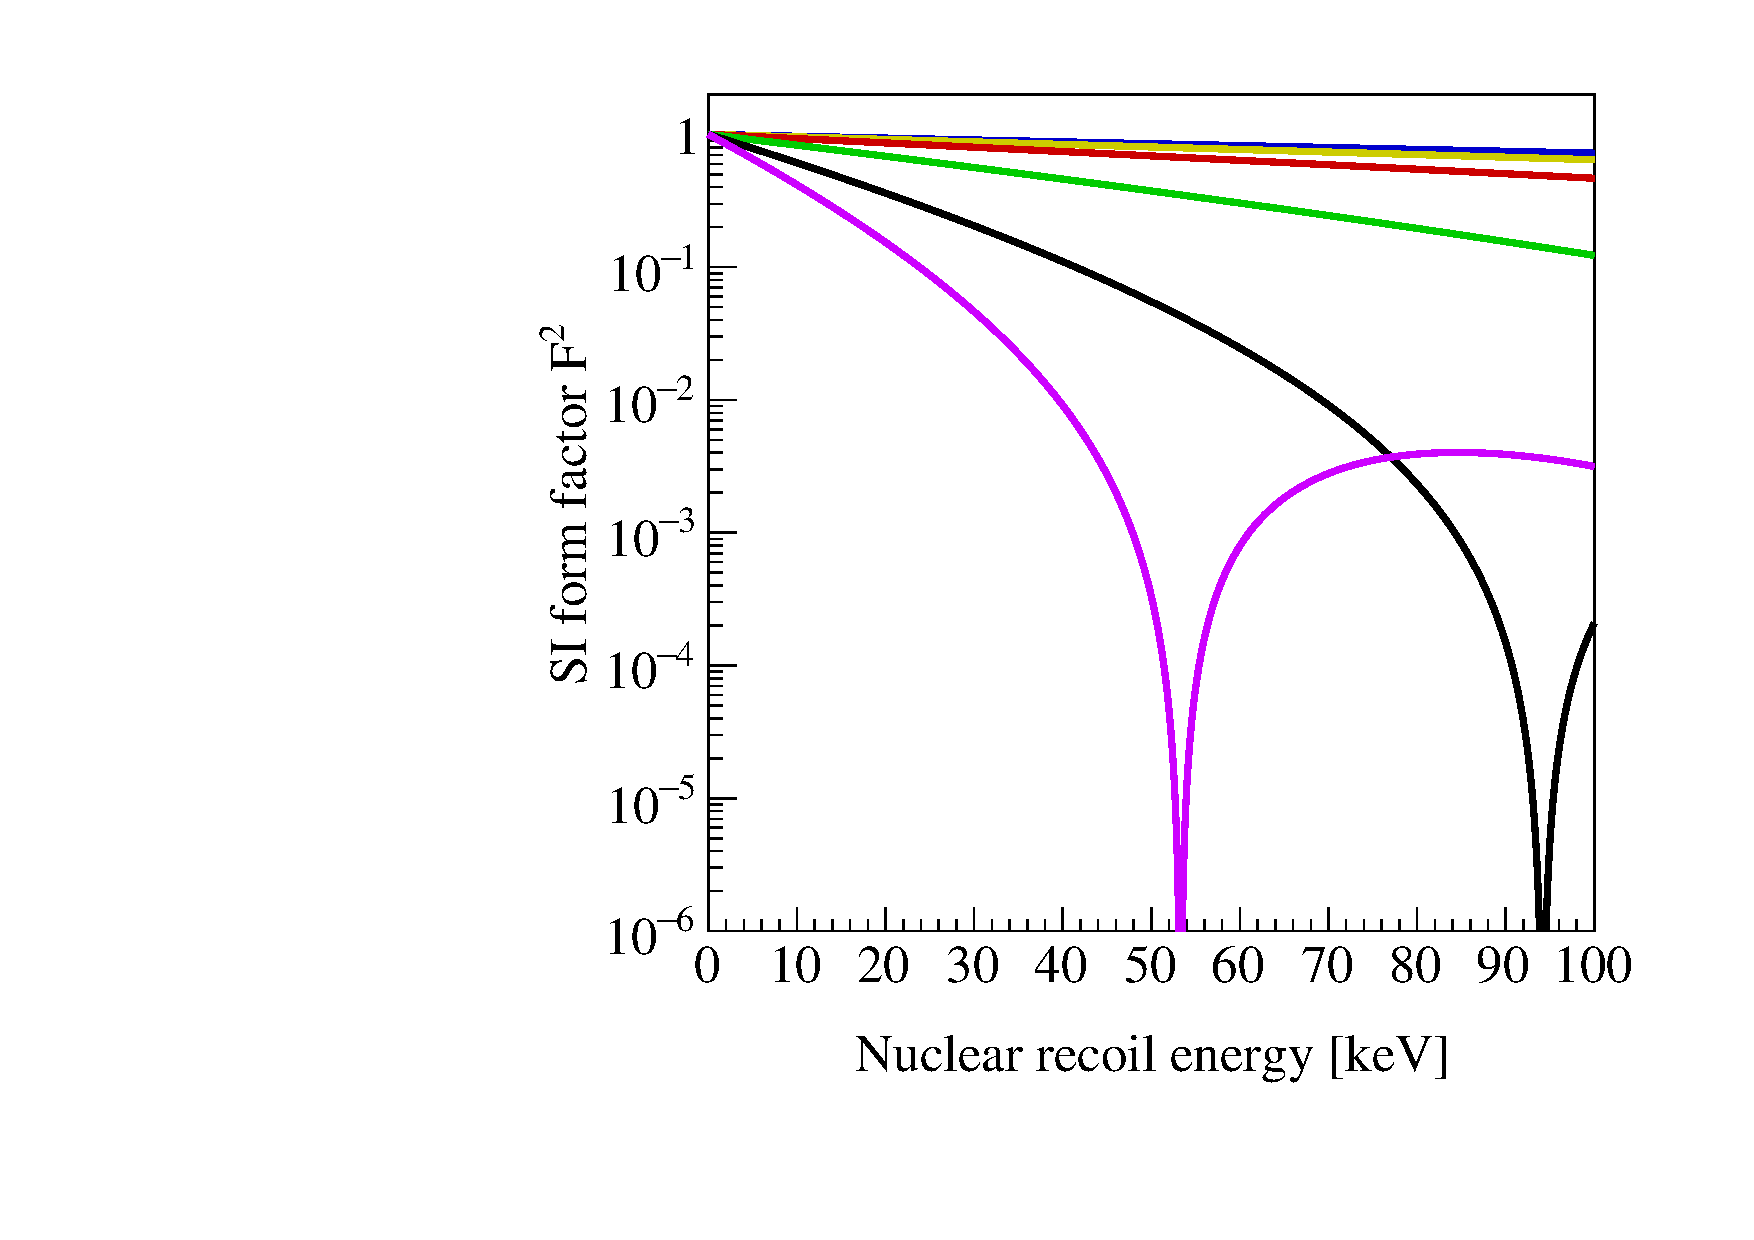
\includegraphics[width=\textwidth]{figures/DMOverview/wimp_event_rate_si_m100_ff.pdf}
         \caption{}
         \label{fig:DMOverview/SIFF}
     \end{subfigure}
     \caption[The spin-independent differential event rate and the spin-independent nuclear form factor as a function of nuclear recoil energy for different target elements.]{\textbf{Left:} The spin-independent differential event rate as a function of nuclear recoil energy for different target elements. A WIMP mass of 100~GeV/$c^2$, a WIMP-nucleon cross-section of $\sigma^\text{SI}_n=1~\text{zb}$, and standard halo model WIMP velocity distribution are assumed. \textbf{Right:} The spin-independent nuclear form factor as a function of nuclear recoil energy for the same sample of elements found in the left panel. Figures reprinted from Ref.~\cite{OlcinaSamblas:thesis}}
     \label{fig:DMOverview/SINRRandFF}
\end{figure}

\paragraph{\textit{A note on search complementarity:}} Direct, indirect, and collider searches for dark matter offer complementary approaches, each with distinct advantages and limitations. Each method relies on the assumption that dark matter interacts with SM particles through a mediator. Therefore, a signal observed in one type of experiment should, in principle, be confirmed by the other. Collider searches, however, are constrained by the beam energy (limiting the mass range of detectable dark matter particles) and by the collider's luminosity (which affects the intensity of collisions) but have the capability to access dark matter models via a greater number of interactions.

In contrast, NR signals in direct detection experiments depend less strongly on the dark matter mass and the sensitivity is driven by the exposure of the detector. This makes current direct detection experiments more sensitive to higher mass dark matter when compared to the collider search counterparts. However, the ability to upgrade the search is limited for direct detection experiments by increasing the mass of the detector and livetime. Whereas collider experiments, on the other hand, can be upgraded through technological advances that lead to high beam energies and luminosities.

Indirect detection is similar to direct detection with respect to the interaction couplings that can be probed; however, searches for the decay products of dark matter self-annihilation suffer from background contamination, as many of the signals may also be produced by known astrophysical sources.

An overview of the individual strengths of each of the different detection approaches is shown in \autoref{tab:DMOverview/interactions} and their ability to access dark matter via different couplings and interactions. Whilst direct and indirect are not as sensitive to all couplings collectively, their searches extend far beyond the current capabilities of collider searches \cite{Penning:2017tmb}.
\begin{table}[h!]
\centering
\small

\newcolumntype{C}[1]{>{\centering\let\newline\\\arraybackslash\hspace{0pt}}m{#1}}
\begin{tabular}{C{1cm}|C{5.cm}|C{5.cm}|}
    
    \rotatebox{90}{\textit{~EW couplings}} \rotatebox{90}{~(Spin 1)~}& {\textbf{Vector:}} \newline $g_{\textrm{DM}} Z'_{\mu} \bar{\chi}\gamma^{\mu}\chi $ \newline Direct detection more sensitive than colliders except at very low dark matter masses.  & {\textbf{Axial-Vector:}} \newline $g_{\textrm{DM}} Z'_{\mu} \bar{\chi}\gamma^{\mu}\gamma^5\chi $ \newline Direct detection and colliders are about equally sensitive in different regions of parameter space.
\\ \hline
     \rotatebox{90}{~\textit{Yukawa couplings}~} \rotatebox{90}{~(mass dependent)~} & {\textbf{Scalar}}: \newline $g_{\textrm{DM}} S\bar{\chi}\chi $ \newline Direct detection and collider about equally sensitive in different regions of parameter space. 
 & {\textbf{Pseudo-Scalar}}:\newline  $g_{\textrm{DM}} S\bar{\chi}\gamma^5\chi $ \newline 
 No limits from direct detection, only from indirect. Colliders provide limits comparable to scalar couplings.
 
\end{tabular}
\caption[Overview of the relative sensitivities of the three main dark matter detection mechanisms.]{Overview of the relative sensitivities of the three main dark matter detection mechanisms. All three approaches are required to cover the maximal phase space. Adapted from Ref.~\cite{Penning:2017tmb}.\label{tab:DMOverview/interactions}}
\end{table}

\subsubsection{Direct detection approaches}
The direct detection of dark matter aims to observe nuclear or electronic recoils resulting from interactions between the dark matter particle and the target material within a detector. These interactions are expected to produce recoil energies in the range of $1-100\,\mathrm{keV}$, assuming incident dark matter particles with masses between $10-1000\,\mathrm{GeV}/c^2$~\cite{DirectDetection2015}. The resulting signals from such recoils can be observed in one or more of three forms: phonons (heat), ionization (charge), and scintillation (light). Detectors are therefore typically designed to be sensitive to one or two of these signal channels, depending on the detection strategy employed. A schematic representation of this detection process is shown in \autoref{fig:DMOverview/DirectDetectorTriangle}, and each of the different direct detection technologies is outlined below:
\begin{figure}[ht!]
	\centering
	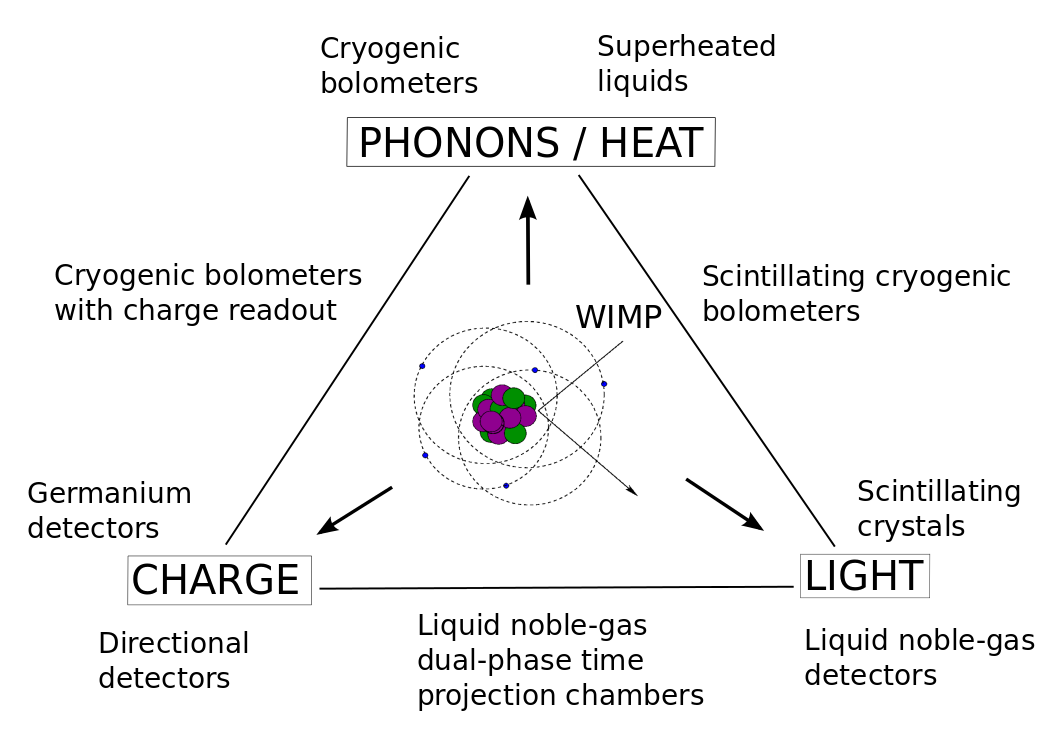
\includegraphics[width=0.6\textwidth]{figures/DMOverview/Direct_direction.png}
	\caption[A schematic showing the possible direct detection signals with corresponding experiments.]{A schematic showing the possible direct detection signals and the corresponding experiments used to observe such signals. Figure reprinted from Ref.~\cite{DirectDetection2015}.}
	\label{fig:DMOverview/DirectDetectorTriangle}
\end{figure}
\begin{itemize}
    \item \textbf{Anorganic Crystal Detectors} use $\mathcal{O}(1)$kg-scale arrays of high-purity scintillator crystals, mainly NaI(Tl) but also CsI(Tl), which are monitored by low-background photomultiplier tubes (PMTs), shown schematically in \autoref{fig:DMOverview/crystal}. The high mass numbers of I ($A=127$) and Cs ($A=133$) lead to a high sensitivity to spin-independent interactions \cite{Schumann:2019eaa}. However, they lack position reconstruction capabilities, which prevents fiducialisation discrimination and results in relatively high background levels. Consequently, WIMP searches using this technology focus on detecting annual modulations in low-energy signals, which arise from the Earth’s changing velocity relative to the Solar System's motion through the dark matter halo. Experiments which rely on this type of detector technology include DAMA/LIBRA \cite{DAMA:2008jlt} and COSINE-100 \cite{COSINE-100:2019lgn}. If a bias voltage is applied across the crystal, charge rather than scintillation is read out; an example of a charge readout detector is DAMIC \cite{Privitera:2024tpq}.
    
    \item \textbf{Cryogenic Crystal Detectors} operate via the detection of the heat signal in the form of phonons, which is measured through the increase in temperature following a particle interaction within the crystalline detector. The sensitivity to record the increase in temperature from an energy deposit is dependent on the detector's heat capacity and how well the detector couples to the heat bath. These detectors are operated at cryogenic temperatures (typically $\leq50~\text{mK}$) to minimize thermal noise and enhance sensitivity. Dielectric crystals such as Ge and Si are particularly well-suited for cryogenic operation as their heat capacity is given by $C \propto M \times T^3$ below their Debye temperature, which is well above room temperature for Ge and Si, where $M$ denotes the mass of the detector \cite{Schumann:2019eaa}. Transition Edge Sensors (TES) are used to detect the tiny temperature rise. The TES is operated at the transition temperature between its superconducting and the normal-conducting state, where a small temperature change will result in a large change in resistivity of the wire and subsequent current flowing through the wire in contact with the crystal. An alternative detector is neutron transmutation doped (NTD) germanium thermistors whose resistivity strongly depends on the temperature \cite{Schumann:2019eaa}. 
    
    Applying both of these detector readout methods allows for signal/background discrimination in a WIMP search, as the partition of the signal into the two channels depends on the recoil type \cite{PhysRevLett.69.3425}. This concept is demonstrated in \autoref{fig:DMOverview/cryogenic} and has been adopted by all modern cryogenic experiments. As the detectors need to be operated at mK temperatures, this can be challenging \& expensive, and the mass of a single detector is limited to kg-scale due to small heat capacity requirements. The latter is overcome by using arrays of crystals; however, this comes with its own challenges, as the high surface-to-volume ratio of such an experiment is not optimal, and surface contamination has to be rejected. Some notable collaborations are SuperCDMS \cite{SuperCDMS:2014cds}, EDELWEISS \cite{Benoit:2002hf} and TESSERACT \cite{TESSERACT:2025tfw}.
    
    \item \textbf{Bubble Chambers} use superheated liquids, usually refrigerants such as CF$_3$I or C$_3$F$_8$ as the WIMP target \cite{Schumann:2019eaa}. The liquids are kept at a temperature near their boiling point, maintaining a `superheated' state. An energy deposition above the detector threshold (as low as 3.3~keV) produces a local phase transition which results in the formation of a bubble. The probability of bubble formation is dependent on the energy loss $dE/dx$ of the particle, and the detector can be tuned such that the only nuclear recoil $\alpha$, neutrons, or WIMP events create bubbles. This property of the bubble chamber means that the electronic recoil background is very heavily suppressed ($< 10^{-9}$). After each bubble has formed, the chamber must be compressed to remove the bubble and then decompressed to return the liquid to a superheated state. This detector recuperation process is time-consuming and induces long detector deadtime and a complicated calibration process. Additionally, bubble chambers do not provide any energy reconstruction capability, as every energy deposition above the detector threshold will result in a bubble. The signal produced in a bubble chamber is read out by a camera arranged stereoscopically, which is triggered by acoustic sensors that allow for precise 3D position reconstruction \cite{edfraser:thesis}, a schematic of the experimental setup is shown in \autoref{fig:DMOverview/bubble}. Examples of collaborations which use this detector are PICASSO \cite{Behnke:2016lsk} and PICO \cite{PICO:2015pux}.
    
    \item \textbf{Directional Detectors} search for excesses of events in the average direction of the WIMP wind through track reconstruction. As the Earth rotates once a day with respect to the expected WIMP flux, daily modulation of the signal is expected. To indicate the direction of the WIMP flux, detectors must have precise track reconstruction capabilities. As the nuclear recoil’s track length depends on the target density, a longer track facilitates the reconstruction of the track direction \cite{Schumann:2019eaa}. Directional detectors employ low-pressure gas targets, most commonly $\text{CF}_4$, with fine-granularity track readout in a Time Projection Chamber (TPC) geometry, as shown in \autoref{fig:DMOverview/directional}. Electronic recoil backgrounds are heavily suppressed based on longer tracks and lower ionisation density. An example of collaboration using this form of detector is DRIFT \cite{BATTAT201765}.

    \item \textbf{Noble Liquid Detectors} use argon and xenon as they are both ionized easily, excellent scintillators, and can be liquefied to create compact and dense dark matter targets. Krypton has similar properties, but due to its high intrinsic background from long-lived isotopes, it is not considered for dark matter searches. Particle interactions in liquid noble gases produce excited, X$^*$ and ionised atoms, X$^+$, as well as heat (which is not detected). The X$^*$ atom combines with a neutral atom to form excimer states, X$^*_2$, which decay, resulting in the emission of ultraviolet light:
    \begin{equation}\label{eqn:DMOverview/scint}
        \textnormal{X}^*  \xrightarrow{+\textnormal{X}} \textnormal{X}^*_2 \rightarrow 2\, \textnormal{X} + h \nu
    \end{equation}
    The light has wavelengths of 128~nm and 178~nm for argon and xenon, respectively. Photo-sensors currently can detect xenon scintillation light, but this is not the case for argon. Wavelength shifters such as tetraphenyl butadiene (TPB) are employed to shift the wavelength of light to optical wavelengths, blue light at 425~nm. 
    
    Noble liquid detectors can be separated into two categories \textit{single-phase} detectors and \textit{dual-phase} detectors.

    \textbf{Single-phase noble liquid detectors} are sensitive to WIMPs through the detector mechanism outlined in \autoref{eqn:DMOverview/scint}, and measure scintillation light using PMTs which surround a spherical target in a $4\pi$ geometry as shown in \autoref{fig:DMOverview/singlephase}. Position of the particle interaction is determined using photon timing and signal distribution in the PMT array, with a typical resolution of a few cm. Backgrounds are suppressed using pulse-shape discrimination in argon-based detectors, whereas xenon-based detectors are limited to target fiducialisation, taking advantage of xenon's self-shielding properties. Notable examples of single-phase noble liquid detectors include XMASS \cite{Abe:2013tc} and DEAP-3600 \cite{DEAP-3600:2024szw}.

    \textbf{Dual-phase noble liquid detectors} operate in a cylindrical geometry with two PMT arrays, as illustrated in \autoref{fig:DMOverview/dualphase}. Signal production via excitation and ionization is discussed further in \autoref{sec:LZ/LXeTPC}, along with recoil-type discrimination for background suppression, and the components for the LZ TPC are shown in \autoref{fig:LZ/CAD_TPC}. Key experiments using this approach include LUX-ZEPLIN (LZ) \cite{LZNIMA}, XENON \cite{XENON:2025vwd}, DARKSIDE \cite{DarkSide-20k:2017zyg}, and PANDA-X \cite{PandaX-4T:2021bab}.
\end{itemize}
\noindent
The three signal channels, phonons, charge, and light, are employed across a range of experimental approaches that collectively cover the parameter space where WIMP interactions are expected. Should any one technique observe a potential dark matter signal, independent confirmation using one or more of the other detection methods would be essential to establish the robustness of the result.

\pagebreak

\begin{figure}[!h]
     \centering
     \begin{subfigure}{0.49\textwidth}
         \centering
         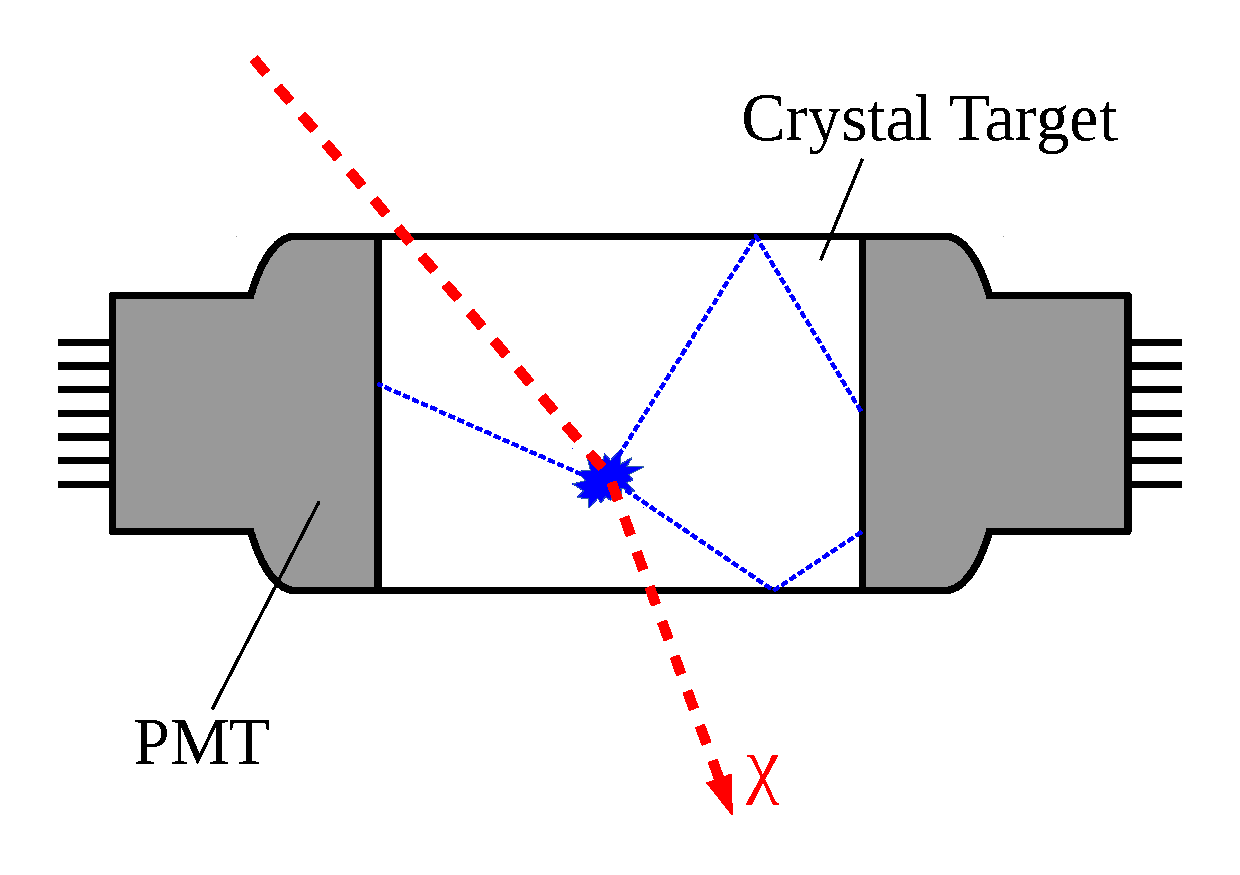
\includegraphics[width=\textwidth]{figures/DMOverview/crystal.pdf}
         \caption{}
         \label{fig:DMOverview/crystal}
     \end{subfigure}
     \hfill
     \begin{subfigure}{0.49\textwidth}
         \centering
         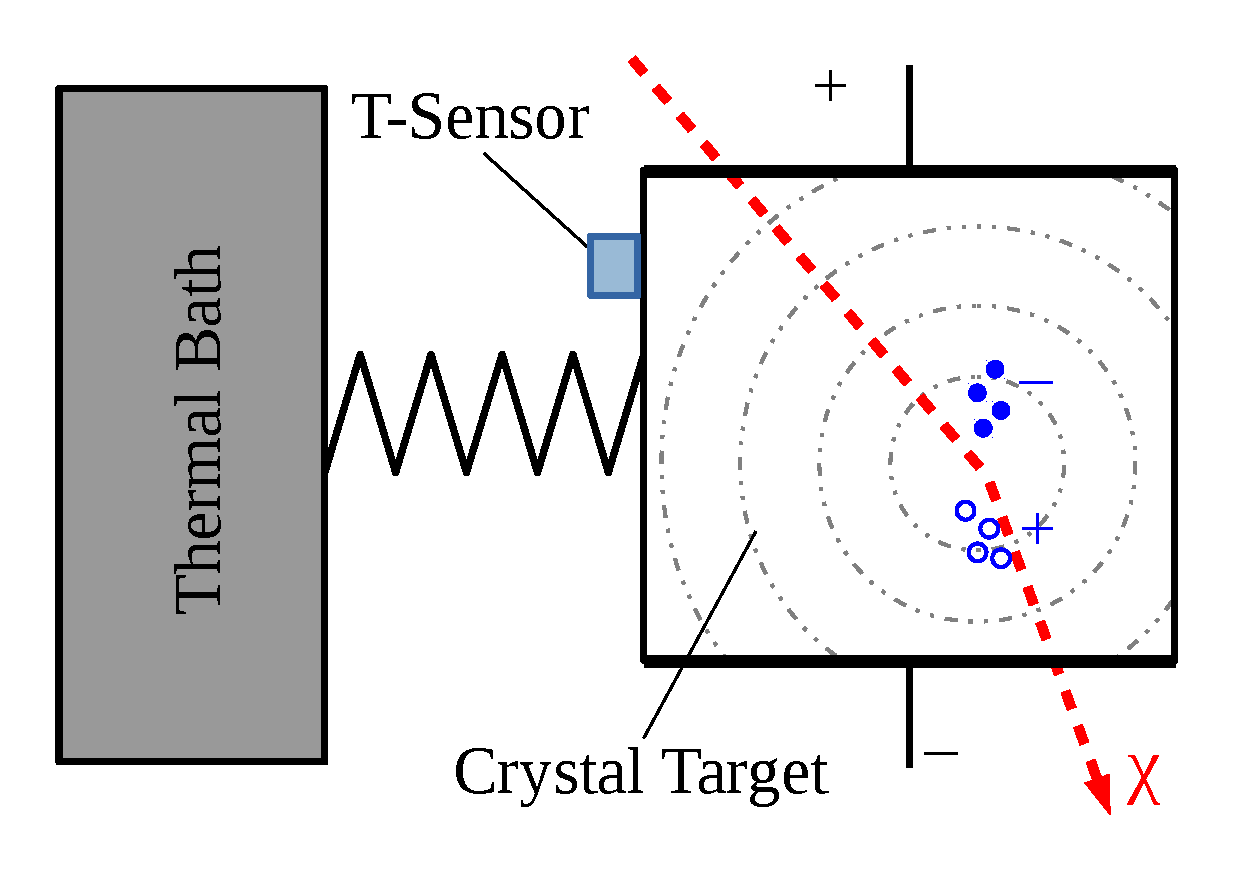
\includegraphics[width=\textwidth]{figures/DMOverview/cryogenic.pdf}
         \caption{}
         \label{fig:DMOverview/cryogenic}
     \end{subfigure}
     \hfill
     \begin{subfigure}{0.49\textwidth}
         \centering
         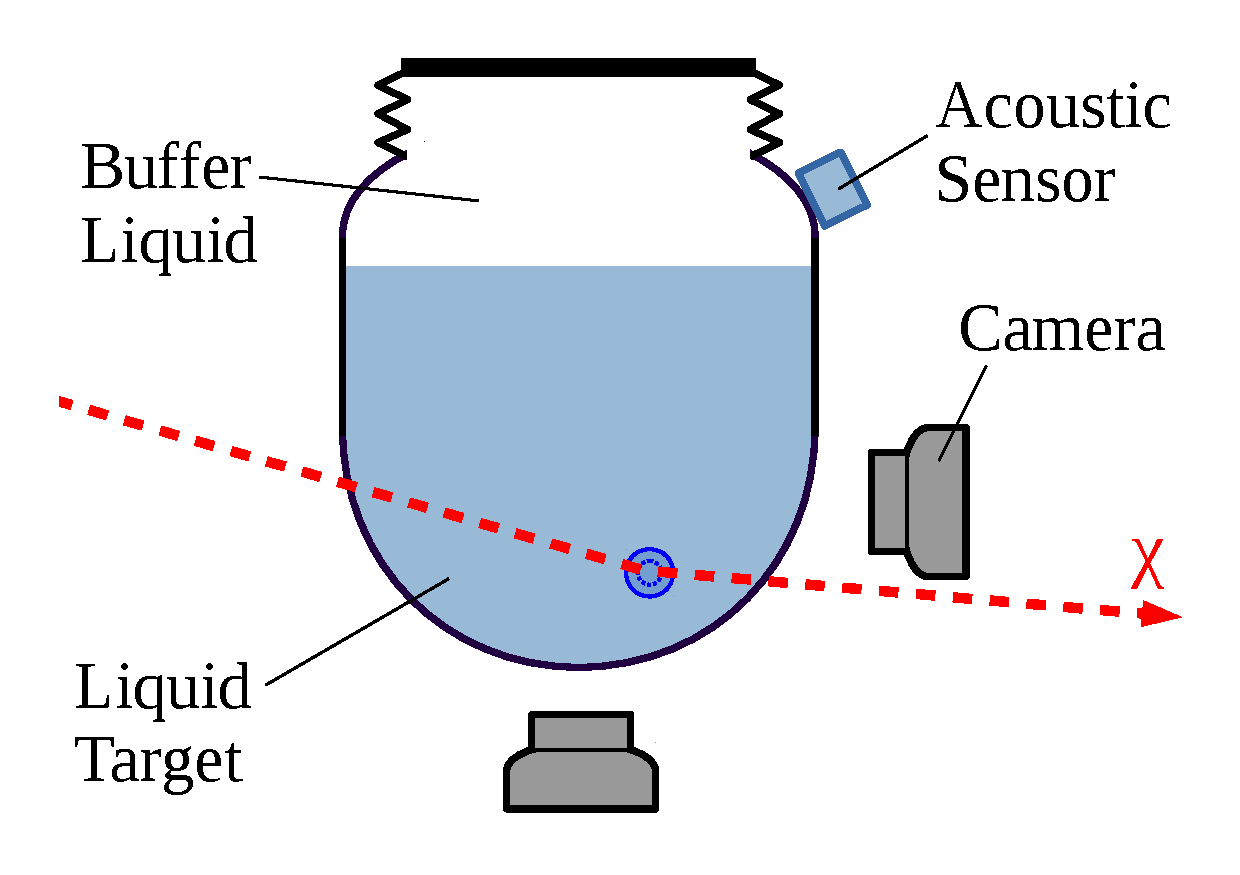
\includegraphics[width=\textwidth]{figures/DMOverview/bubble.pdf}
         \caption{}
         \label{fig:DMOverview/bubble}
     \end{subfigure}
     \hfill
     \begin{subfigure}{0.49\textwidth}
         \centering
         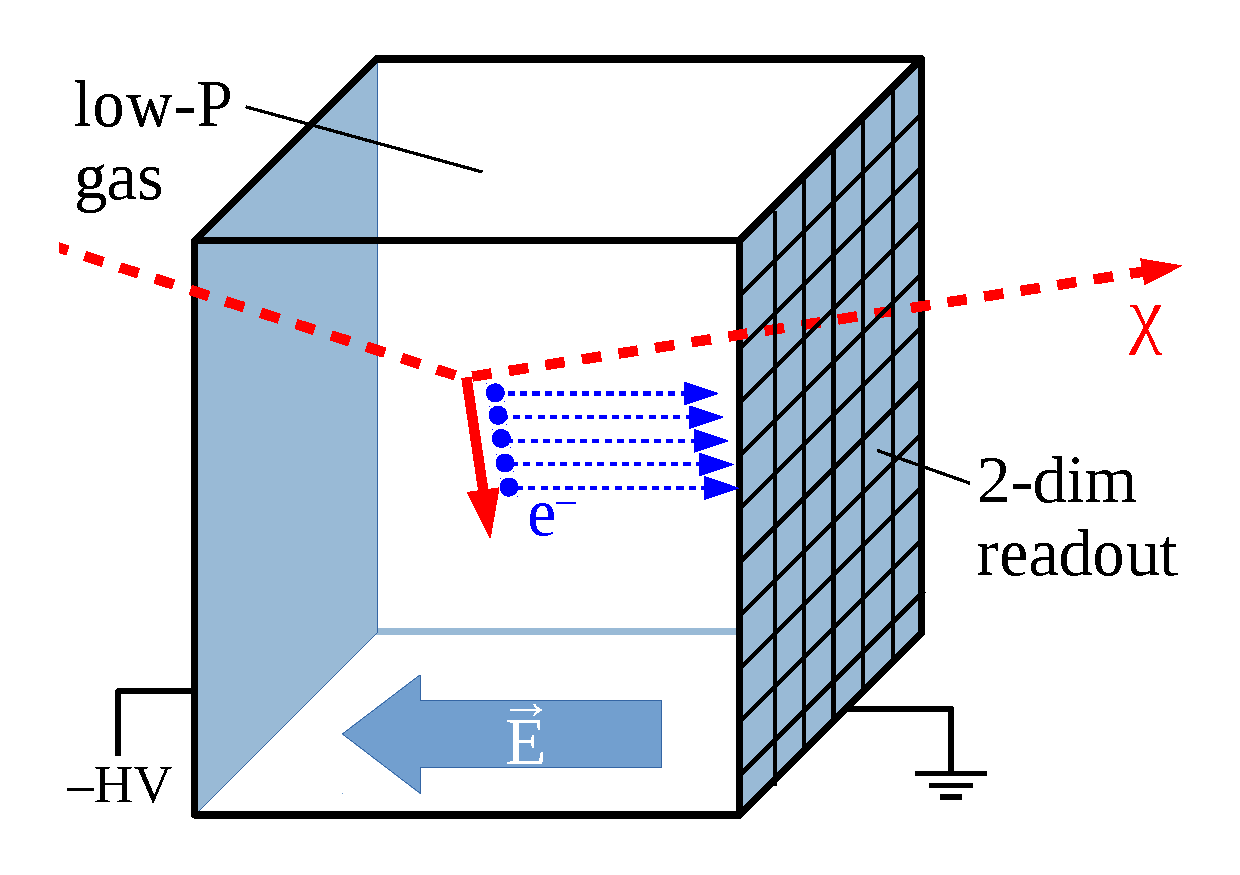
\includegraphics[width=\textwidth]{figures/DMOverview/directional.pdf}
         \caption{}
         \label{fig:DMOverview/directional}
     \end{subfigure}
     \hfill
     \begin{subfigure}{0.49\textwidth}
         \centering
         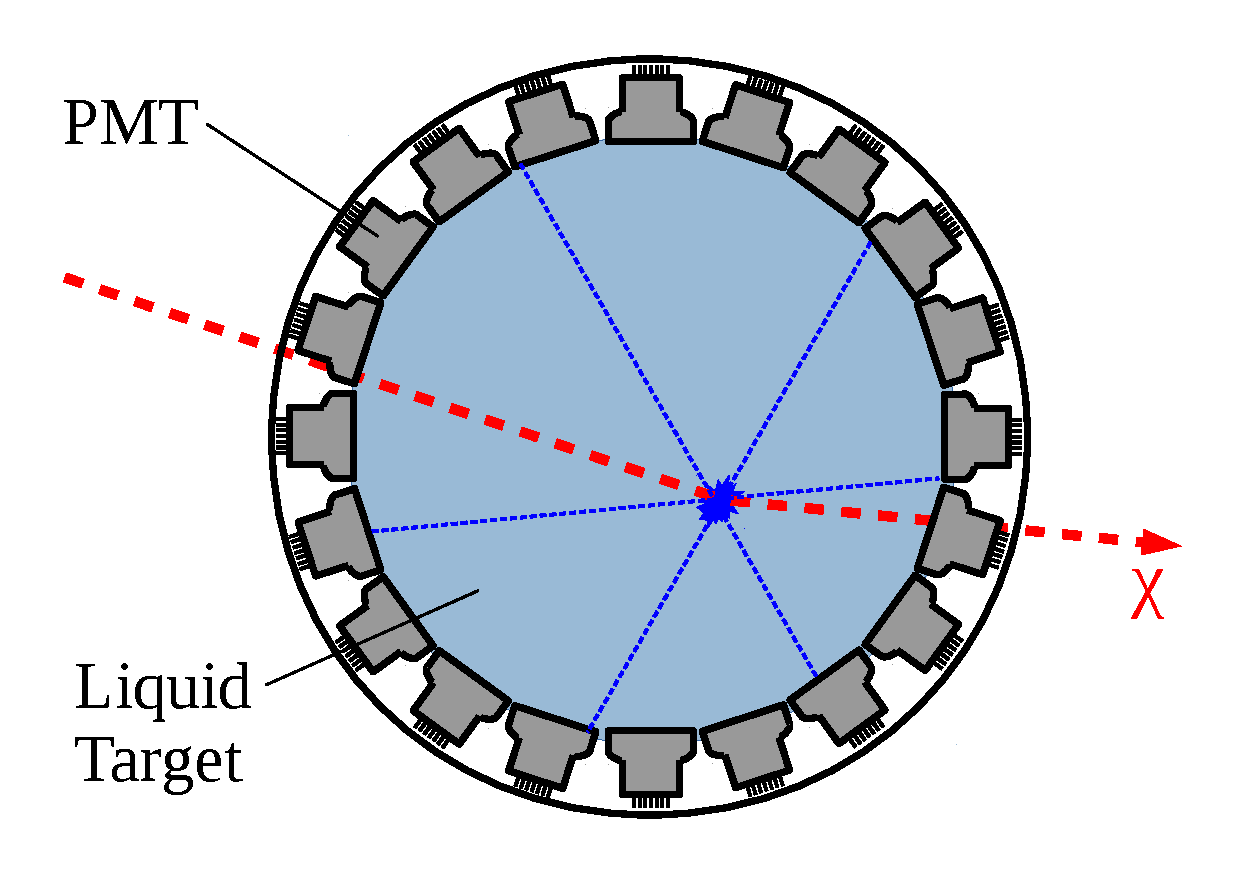
\includegraphics[width=\textwidth]{figures/DMOverview/singlephase.pdf}
         \caption{}
         \label{fig:DMOverview/singlephase}
     \end{subfigure}
     \hfill
     \begin{subfigure}{0.49\textwidth}
         \centering
         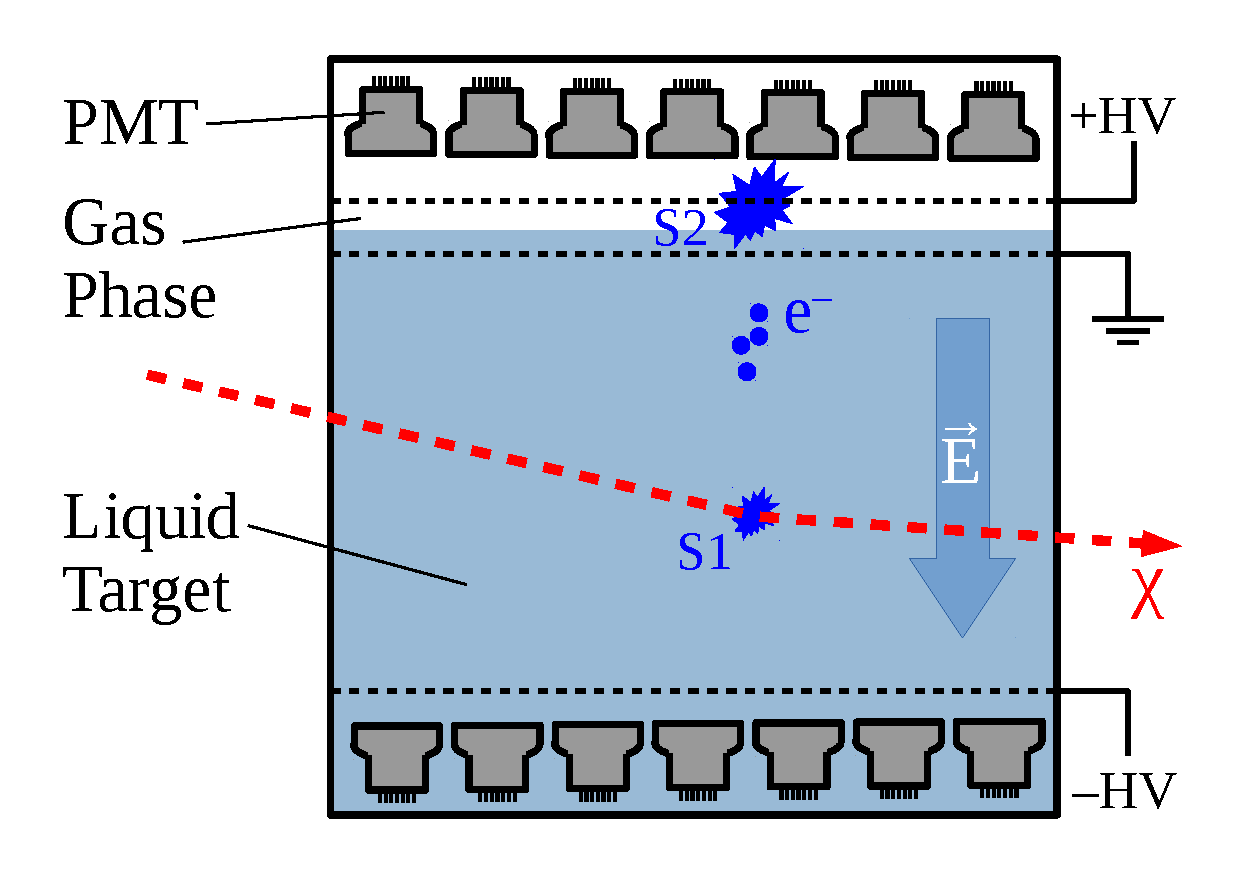
\includegraphics[width=\textwidth]{figures/DMOverview/dualphase.pdf}
         \caption{}
         \label{fig:DMOverview/dualphase}
     \end{subfigure}
     \caption[Schematics of signal readout in different direct detection experiments.]{Schematics of signal readout in different direct detection experiments upon nuclear recoil with dark matter particle $\chi$ (red dashed arrow). Areas of blue indicate a liquid target, white indicates the remaining crystal and gas targets and grey area represents some energy detection device. All figures reprinted from Ref.~\cite{Schumann:2019eaa}.}
     \label{fig:DMOverview/DDSetups}
\end{figure}

\pagebreak

\subsubsection{Current status for WIMP dark matter direct searches}\label{sec:DMOverview/DMCurrentStatus}
At the time of writing, no experiment has detected a dark matter particle. However, stringent upper limits on the WIMP–nucleon interaction cross-section have been established by xenon TPCs, particularly in the mass range around $m_\chi \approx 40~\text{GeV}/c^2$. The most recent spin-independent WIMP–nucleon cross-section limits as a function of WIMP mass are shown in \autoref{fig:DMOverview/WIMPCrossSec.pdf}. Also shown in this figure is the coherent neutrino–nucleus scattering background, which defines a fundamental sensitivity limit for direct detection experiments. As dark matter detectors grow in size and accumulate exposure, they become increasingly sensitive to neutrinos from astrophysical sources, which can closely mimic genuine WIMP signals \cite{Billard:2013qya}. Without new methods of background discrimination, this so-called \textit{neutrino fog} may represent the ultimate limit of sensitivity in this mass range for current detection technologies \cite{Boehm:2018sux}. At WIMP masses below a GeV, the best constraints have been achieved by small-scale ultra-sensitive detectors with very low detection thresholds \cite{mwilliams:thesis}. Target materials such as helium \cite{SPICE:2023tru}, silicon \cite{TESSERACT:2025tfw,DAMIC:2020cut}, and germanium \cite{SuperCDMS:2017nns} are favoured for such searches.

The remaining viable parameter space for GeV-scale dark matter is currently being explored by several experiments. The XENON, PandaX, and LZ collaborations have led the search for WIMPs over the past two decades and are expected to further improve current upper limits by an order of magnitude within the next three years. Planning is already underway for a next-generation liquid xenon observatory (XLZD), which aims to probe WIMP parameter space down to the neutrino fog, with a projected $3\sigma$ discovery potential for cross-sections as low as $3\times10^{-49}\,\text{cm}^2$ \cite{XLZD:2024nsu}. The baseline design of the detector will have an active liquid xenon target of 60 tonnes, with the potential to be increased to 80 tonnes. The detector will be based on mature liquid xenon dual-phase time projection chamber (TPC) technologies used in current-generation experiments. Global R\&D efforts are currently ongoing to support the development of the proposed large-scale TPC \cite{Brown:2023vgf,Baudis:2023ywo}.

In the remainder of this thesis, I will focus on the LZ experiment, specifically the commissioning of its Outer Detector, the optimisation of its active neutron veto system, quantifying its veto system's performance, and a measurement of the atmospheric muon flux. While WIMPs are expected to interact only with the xenon target, neutrons, one of the dominant backgrounds in a WIMP search, can interact in both the TPC and veto systems. Neutrons are produced via a number of mechanisms \cite{Kudryavtsev:2020eer}, one of which is through muon-induced cascades in materials surrounding the detector. The measurement of the muon flux through LZ is a key component in the determination of muon-induced neutrons and the resulting neutron background \cite{LZ:2022ysc}. Neutrons produced through spontaneous fission and ($\alpha$,n) reactions in detector components are the dominant source of detector nuclear recoils in the background model \cite{LZ:2024zvo,LZ:2022ysc}. The ability of active veto system to identify such events and in turn reject these events is one of the key factors that establishes LZ as the leading dark matter experiment of its kind today \cite{LZ:2024zvo}. 

\begin{figure}[ht!]
    \centering
    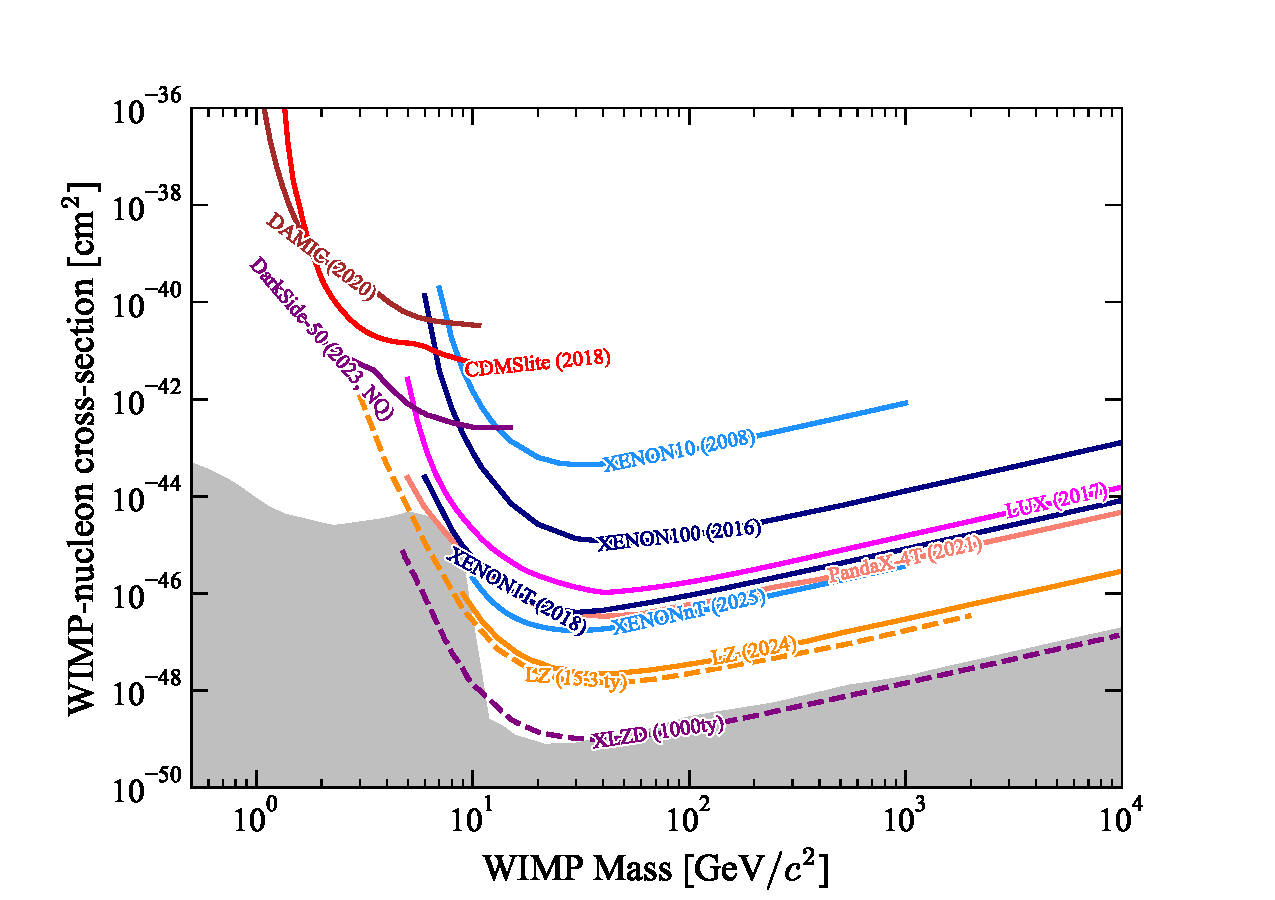
\includegraphics[width=\linewidth]{figures/DMOverview/allwimp_limits.pdf}
    \caption[Most recent spin-independent WIMP-nucleon cross section limits as a function of WIMP mass.]{Most recent spin-independent WIMP-nucleon cross section limits as a function of WIMP mass for direct detection experiments alongside projected limits for current and future experiments. Figure produced using Ref.~\cite{DDLimitRepo} includes limits from DAMIC \cite{DAMIC:2020cut}, CDMSlite \cite{SuperCDMS:2017nns}, Darkside 50 \cite{DarkSide:2018bpj}, XENON10 \cite{XENON:2007uwm}, XENON100 \cite{XENON100:2016sjq}, LUX \cite{LUX:2016ggv}, PandaX-4T \cite{PandaX-4T:2021bab}, XENON1T \cite{XENON:2018voc}, XENONnT \cite{XENON:2025vwd}, LUX-ZEPLIN (LZ) experiment \cite{LZCollaboration:2024lux}. Projected limits shown have been produced by LZ \cite{LZ:2018qzl} and XLZD \cite{XLZD:2024nsu}. The area coloured in grey represents the neutrino floor \cite{Billard:2013qya}.}
    \label{fig:DMOverview/WIMPCrossSec.pdf}
\end{figure}